\chapter{Úvod}

Porozumenie cudzím myšlienkam býva občas zložité. Správne podať svoj názor alebo ideu je o to ťažšie, ak sme odkázaní len na verbálne vyjadrovacie prostriedky. Nie každý sa narodil s darom reči, či s dostatočnou dávkou sebavedomia pre verejné vystupovanie. Hoci sa tieto schopnosti dajú nadobudnúť dlhodobým tréningom, niekedy aj najskúsenejší rečník potrebuje použiť inú formu vyjadrovania. Veď nie nadarmo sa hovorí, že obrázok je hodný tisíc slov.

Ešte pred pár desiatkami rokov si rečník musel vystačiť sám, avšak s nástupom nových technológií sa toto obmedzenie vytratilo. Premietanie priesvitiek na plátno dodalo prezentáciám nový rozmer. Rečník tak mohol lepšie a rýchlejšie zachytiť podstatu prezentovanej myšlienky, než by to bolo možné predtým. Hoci sa priesvitky pomaly vytrácajú, ako väčšina zastaralých technológií si však stále nájdu svojich priaznivcov.

S príchodom osobných počítačov a projektorov sa situácia opäť zmenila. Priesvitky sa zdigitalizovali, zmenili meno, vznikli programy určené na ich jednoduchú tvorbu a odrazu všetci mohli podať vizuálne dokonalú prezentáciu. O~rečníckej časti sa to žiaľ povedať nedá.

Slajdy, ako sa dnes nazývajú novodobé priesvitky, dostali mnoho funkcií. Možnosť vložiť multimediálny obsah ako obrázky, videá, grafy, či tabuľky je dnes samozrejmosťou. Krásne vizuálne témy idú ruka v ruke s oku lahodiacimi animáciami, či typograficky dokonalým textom.

Hoci počítačové prezentácie nadobudli veľa moderných prvkov, stále sa držia pôvodného konceptu priesvitiek. Tie majú pevný rozmer, ktorý obmedzuje vyjadrenie myšlienky maximálne na pár slajdov. Tento nedostatok je možné prekonať nahradením množstva malých slajdov jedným veľkým plátnom, kde budú umiestnené prezentované informácie. Samotnou prezentáciou bude postupné zobrazovanie výrezov tohto plátna.

\section{Cieľ a obsah práce}

Cieľom tejto bakalárskej práce je popis a funkčná implementácia nového typu prezentačného softvéru, ktorý využíva na prezentáciu informácií tzv. \textit{Zooming User Interface} -- grafické prostredie, kde sú objekty rozmiestnené na nekonečnej virtuálnej ploche, pričom používateľ môže meniť stupeň priblíženia prehliadanej oblasti za účelom zobrazenia viac alebo menej detailov. Aplikácia bude vytvorená s využitím frameworku \textit{QtQuick}.

Tému pre túto záverečnú prácu som si zvolil z osobného presvedčenia, že ZUI používateľské rozhrania sú v mnohých ohľadoch prirodzenejšie, než tie tradičné, ktoré sa v~dnešnej dobe využívajú. Hoci o prezentačné programy nejavím rovnaký záujem, fakt že existuje iba veľmi málo programov na tvorbu prezentácií, ktoré využívajú \textit{Zooming User Interface}, ma presvedčil, že toto bude vhodná téma na záverečnú prácu. Dôvodom pre voľbu frameworku \textit{QtQuick}, bola chuť naplno využiť deklaratívny prístup tvorby aplikácií, ktorý tento nástroj ponúka.

V~prvej kapitole s~názvom \uv{\nameref{ch:prezentacny_softver}} sa venujeme tradičným prezentačným programom, ktoré sa v~dnešnej dobe používajú. V~kapitole \uv{\nameref{ch:zui}} popisujeme a uvádzame významné príklady tohto druhu používateľských rozhraní. Novým typom prezentačného softvéru sa zaoberáme v~kapitole \uv{\nameref{ch:zui_prezentacny_softver}}, kde vymenujeme a popíšeme vybrané implementácie. Kapitola \uv{\nameref{ch:navrh}} obsahuje detailný popis návrhu ZUI prezentačného programu, ktorého implementáciu opíšeme v~nasledujúcej kapitole \uv{\nameref{ch:implementacia}}. V~poslednej kapitole \uv{\nameref{ch:zhodnotenie}}, zhrnieme dosiahnuté výsledky a popíšeme budúce smerovanie projektu.

\chapter{Prezentačný softvér} \label{ch:prezentacny_softver}
\section{Popis} \label{sec:presentation_desc}

Prezentačný softvér alebo jednoducho prezentačný program, je aplikácia, ktorá umožňuje používateľovi vytvoriť prezentáciu. Tá sa typicky skladá z jedného alebo viacerých snímok, ktoré sa nazývajú slajdy (z anglického \textit{slide}). Samotná prezentácia je teda len prepínanie jednotlivých slajdov, ktoré nasledujú za sebou.

Ako budeme môcť vidieť, súčasné prezentačné programy obsahujú rôznorodú funkcionalitu. Avšak používanie slajdov robí z týchto aplikácií doslova len moderné priesvitky.

\section{Existujúce riešenia}

Na svete sa dá nájsť nespočetné množstvo prezentačného softvéru. Máme na výber z~komerčne úspešných produktov, ale aj z~projektov s~otvoreným zdrojovým kódom, ktoré im celkom úspešne konkurujú. V nasledujúcej časti si popíšeme štyri najpoužívanejšie prezentačné systémy.

\subsection{Microsoft PowerPoint} \label{sec:powerpoint}

Jednoznačne najpopulárnejším a najpoužívanejším programom na tvorbu prezentácií je \textit{Microsoft PowerPoint} z kancelárskeho balíku \textit{Microsoft Office}. Tento prezentačný program pôvodne vznikol v roku 1984 pod názvom \textit{Presenter} ako aplikácia pre počítače \textit{Macintosh} od spoločnosti \textit{Apple}. V roku 1987 bol z dôvodu problémov s obchodnou značkou premenovaný na \textit{PowerPoint} a ešte v tom istom roku odkúpený spoločnosťou \textit{Microsoft}.

\textit{PowerPoint} ponúka bohatú funkcionalitu, ktorá zahŕňa definovanie vlastných animácií na slajde, animácie prechodu slajdov, veľmi pokročilé formátovanie textu, vkladanie obrázkov, videí, tabuliek, grafov a veľa ďalšieho. Používateľ si tiež môže môže vybrať z mnoho preddefinovaných grafických tém a vyrobiť tak profesionálne vyzerajúcu prezentáciu podstatne rýchlejšie.

Aj napriek tomu, že \textit{Microsoft PowerPoint} ponúka veľké množstvo funkcií a je jednoznačnou dominantou v oblasti prezentačného softvéru, nemá žiadnu podstatnú výhodu oproti konkurencií.

\begin{figure}
 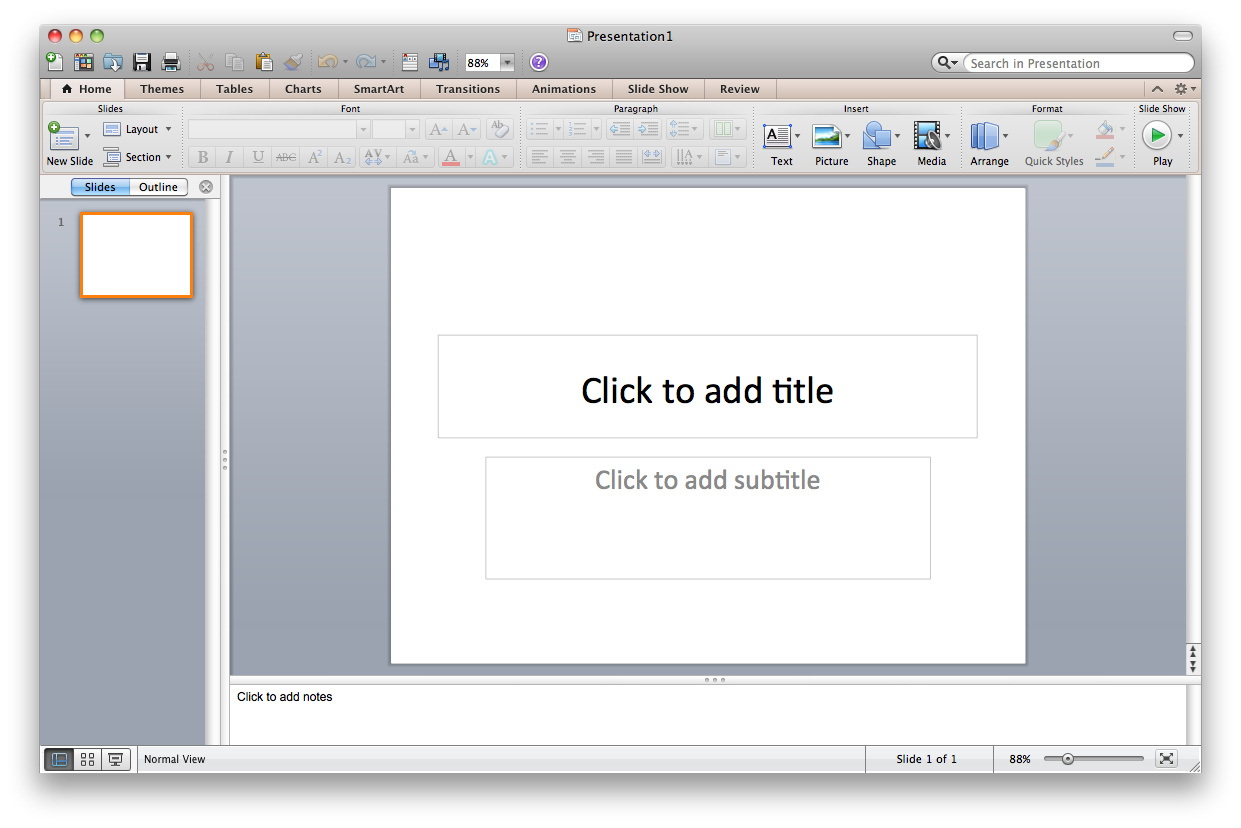
\includegraphics[width=\linewidth]{powerpoint}
 \caption{Microsoft PowerPoint pod Mac OS X\label{fig:powerpoint}}
\end{figure}

\subsection{OpenOffice.org Impress}

\textit{Impress} patrí do slobodného kancelárskeho balíku \textit{OpenOffice.org}, ktorý vznikol na základoch kancelárskeho balíku \textit{StarOffice} od spoločnosti \textit{Sun Microsystems}. Dôvodom vzniku mala byť snaha zapojiť komunitu do vývoja a lepšie konkurovať spoločnosti \textit{Microsoft} s ich balíkom \textit{Office}.

Aplikácia používa na ukladanie prezentácií, tzv. formát \textit{OpenDocument}, ktorý bol schválený a prijatý ako štandard ISO. Okrem podpory natívneho formátu, \textit{Impress} podporuje aj import prezentácií z ostatných prezentačných programov vrátane \textit{Microsoft PowerPoint}.

Po kúpe spoločnosti \textit{Sun Microsystems} v roku 2009 spoločnosťou \textit{Oracle}, sa vyskytli obavy o budúcnosť celého kancelárskeho balíku. Poprední vývojári, ktorý pracovali na balíku, opustili spoločnosť a založili organizáciu \textit{The Document Foundation}, ktorá vytvorila čisto komunitnú vetvu tohto kancelárskeho balíku s názvom \textit{LibreOffice}.

\subsection{Apple Keynote}

\textit{Apple Keynote} patrí do kancelárskeho balíku \textit{iWork} od spoločnosti \textit{Apple}. Podobne ako predchádzajúce dva príklady prezentačných programov, aj \textit{Keynote} používa rovnaký spôsob prezentovania -- slajdy. Hoci sa v tejto základnej črte oproti konkurencií nelíši, obsahuje pár vylepšení, ktoré robia tento produkt zaujímavejším.

Pravdepodobne najzvláštnejšou funkciou, ktorú \textit{Keynote} ponúka je možnosť využiť \textit{iPhone} (smarfón od spoločnosti \textit{Apple}) ako dodatočný displej, ktorý je synchronizovaný s prezentáciou a zobrazovať na ňom poznámky k aktuálnemu slajdu. Samozrejmosťou je možnosť prechádzať medzi jednotlivými snímkami prezentácie jednoduchými gestami na ploche telefónu.

Ďalšou vlastnosťou tohto produktu je možnosť používať pokročilé animácie. Príkladom môže byť funkcia \textit{Magic Move}, ktorá interpoluje pozíciu, veľkosť a rotáciu pre objekt, ak sa nachádza na dvoch snímkach prezentácie za sebou.

\subsection{\LaTeX\ Beamer}

Veľmi nezvyčajný spôsob tvorby prezentácií používa systém \LaTeX\ \textit{Beamer}. Narozdiel od predchádzajúcich programov, \textit{Beamer} nie je tzv. WYSIWYG (\textit{What You See Is What You Get}, v doslovnom preklade \uv{čo vidíš, to dostaneš}) editor, ale balíček makier pre \LaTeX, ktoré umožňujú vytvorenie dokumentu určeného na prezentáciu. Používateľ upravuje zdrojový kód prezentácie, ktorý sa neskôr skompiluje do zobraziteľnej podoby.

Narozdiel od predchádzajúcich programov, \textit{Beamer} nepracuje s pojmom slajd. Používateľ vytvára tzv. rámy (z anglického \textit{frame}), do ktorého umiestňuje informácie.  Používateľ má však možnosť nezobraziť všetky informácie v ráme naraz, ale postupne, čím vytvorí sadu slajdov z jedného rámu. Existuje množstvo funkcií, ktoré ovplyvňujú zobrazenie istej informácie na jednotlivých slajdoch, čím sa dá dosiahnuť veľmi komplexné správanie, ktoré by sa v ostatných prezentačných programoch vytváralo zložito.

Okrem zadefinovania slajdov si používateľ môže vybrať z viacero predpripravených animácií, ktoré spríjemňujú zmenu rámu. Podobne ako pri slajdoch, používateľ má plnú slobodu nad tým, ktorá animácia sa má spustiť pri prechode na ľubovoľný slajd.

\chapter{Zooming User Interface} \label{ch:zui}

\section{Popis}

V nasledujúcej kapitole si popíšeme netradičný typ používateľského rozhrania -- \textit{Zooming User Interface}, ktoré vo veľkej miere používa priblíženie a oddialenie pre zobrazovanie informácií.

\subsection{WIMP} \label{sec:wimp}

Väčšina dnešných grafických používateľských rozhraní (\textit{Graphical User Interface - GUI}) používaných na interakciu medzi človekom a počítačom patrí do skupiny tzv. WIMP používateľských rozhraní. Skratka WIMP označuje \textit{\uv{window, icon, menu, pointing device}}, teda \uv{okno, ikona, kontextová ponuka, ukazovacie zariadenie}, čo vyjadruje prvky, ktoré sa používajú v tomto type používateľských rozhraní. Kvôli veľkému rozšíreniu býva WIMP nesprávne označované ako GUI.

Prvé WIMP používateľské rozhranie bolo vyvinuté v roku 1973 vo výskumnom centre PARC spoločnosti Xerox vrámci projektu Xerox Alto. Aj napriek revolučnej myšlienke, WIMP nebolo považované za správny smer vo vývoji užívateľských rozhraní a dlho ostalo nepovšimnuté. O popularizáciu sa postarala až spoločnosť Apple so svojím počítačom Macintosh v roku 1984. Od toho momentu sa WIMP paradigma stala hlavným prúdom tvorby používateľských rozhraní a za posledné tri desaťročia nepodstúpila takmer žiadne zmeny.

\subsection{Post-WIMP}

Hoci WIMP používateľské rozhrania sú pre začiatočníkov s počítačmi veľmi intuitívne vďaka dobrej analógií s objektami zo skutočného sveta \cite{antimac_ui}, tak významnú úlohu začínajú zohrávať aj tzv. post-WIMP používateľské rozhrania, prvýkrát popísané Jakobom Nielsenom v \textit{Noncommand User Interfaces} \cite{noncmd_ui}. Ako z ich názvu vyplýva, snažia sa odpútať od WIMP paradigmy a využívať alternatívne ovládacie prvky pri interakcií s používateľmi. Typickými príkladmi post-WIMP používateľských rozhraní sú napr. počítačové hry, systémy využívajúce virtuálnu realitu, používateľské rozhrania ovládané gestami, či rečou.

Vďaka rozmachu múdrych telefónov tzv. \textit{smartfónov} a najmä ich operačných systémov, sa začínajú post-WIMP používateľské rozhrania používať omnoho častejšie, aj napriek tomu, že na stolových a prenosných počítačoch ostáva WIMP stále štandardom.

\subsection{ZUI}

\textit{Zooming User Interface}\footnote{niekde označované aj ako \textit{Zoomable User Interface}}, skrátene označované ako ZUI, sa zaraďuje medzi post-WIMP grafické prostredia. Charakteristickou črtou rozhrania sú objekty rozmiestnené na nekonečnej virtuálnej ploche, ktorej prehliadanie je možné vďaka zmene stupňa priblíženia, pohybu po ploche a častokrát aj jej natočeniu.

Používateľ má úplnú slobodu nad navigáciou -- nie je obmedzený veľkosťou plátna, ktoré je nekonečné vo všetkých smeroch. Používateľ sa teda môže pohybovať po ploche podľa svojich potrieb bez akýchkoľvek obmedzení.

Obmedzenie nenastáva ani pri priblížení, resp. oddialení zobrazovanej plochy. Rozlíšenie tejto virtuálnej plochy je podobne ako jej veľkosť tiež nekonečná. Táto skutočnosť umožňuje vtesnať do priestoru medzi dva objekty akékoľvek množstvo objektov, čo ponúka naozaj široké možnosti použitia.

\subsection{Sémantické zväčšenie} \label{sec:semantic-zoom}

Sémantické zväčšenie, angl. \textit{semantic zoom}, je funkcia ZUI rozhraní, ktorá umožňuje meniť obsah zobrazovaného objektu v závislosti od úrovne priblíženia. Narozdiel od obyčajného zväčšenia, ak má objekt na svoje zobrazenie iba veľmi malú plochu, nesnaží sa zobraziť všetky informácie, ktoré má v sebe obsiahnuté, ale len tie, ktoré pri danom stupni zväčšenia majú význam. Objekt teda mení svoju podobu na základe prostredia, v ktorom sa nachádza, resp. poskytuje detaily na vyžiadanie.

Ilustračným príkladom môže byť objekt, ktorý predstavuje film. Ak zobrazujeme veľké množstvo takýchto objektov, teda máme oddialený pohľad, stačí zobrazovať obrázok, ktorý reprezentuje daný film. Ak si objekt priblížime, môžeme k obrázku pridať názov filmu. Ak sa priblížime ešte viac, máme už dostatok plochy na zobrazenie textového popisu filmu. Ak bude na ploche viditeľný už len sám objekt, môže sa zobraziť zoznam obsadenia, hodnotenie alebo dokonca aj ukážku z filmu.

Implementáciu popísaného príkladu sémantického zväčšenia je možné nájsť v aplikácií \textit{MedioVis2}, ktorá je vyobrazená na obrázku~\ref{fig:semantic-zoom}.

\begin{figure}
 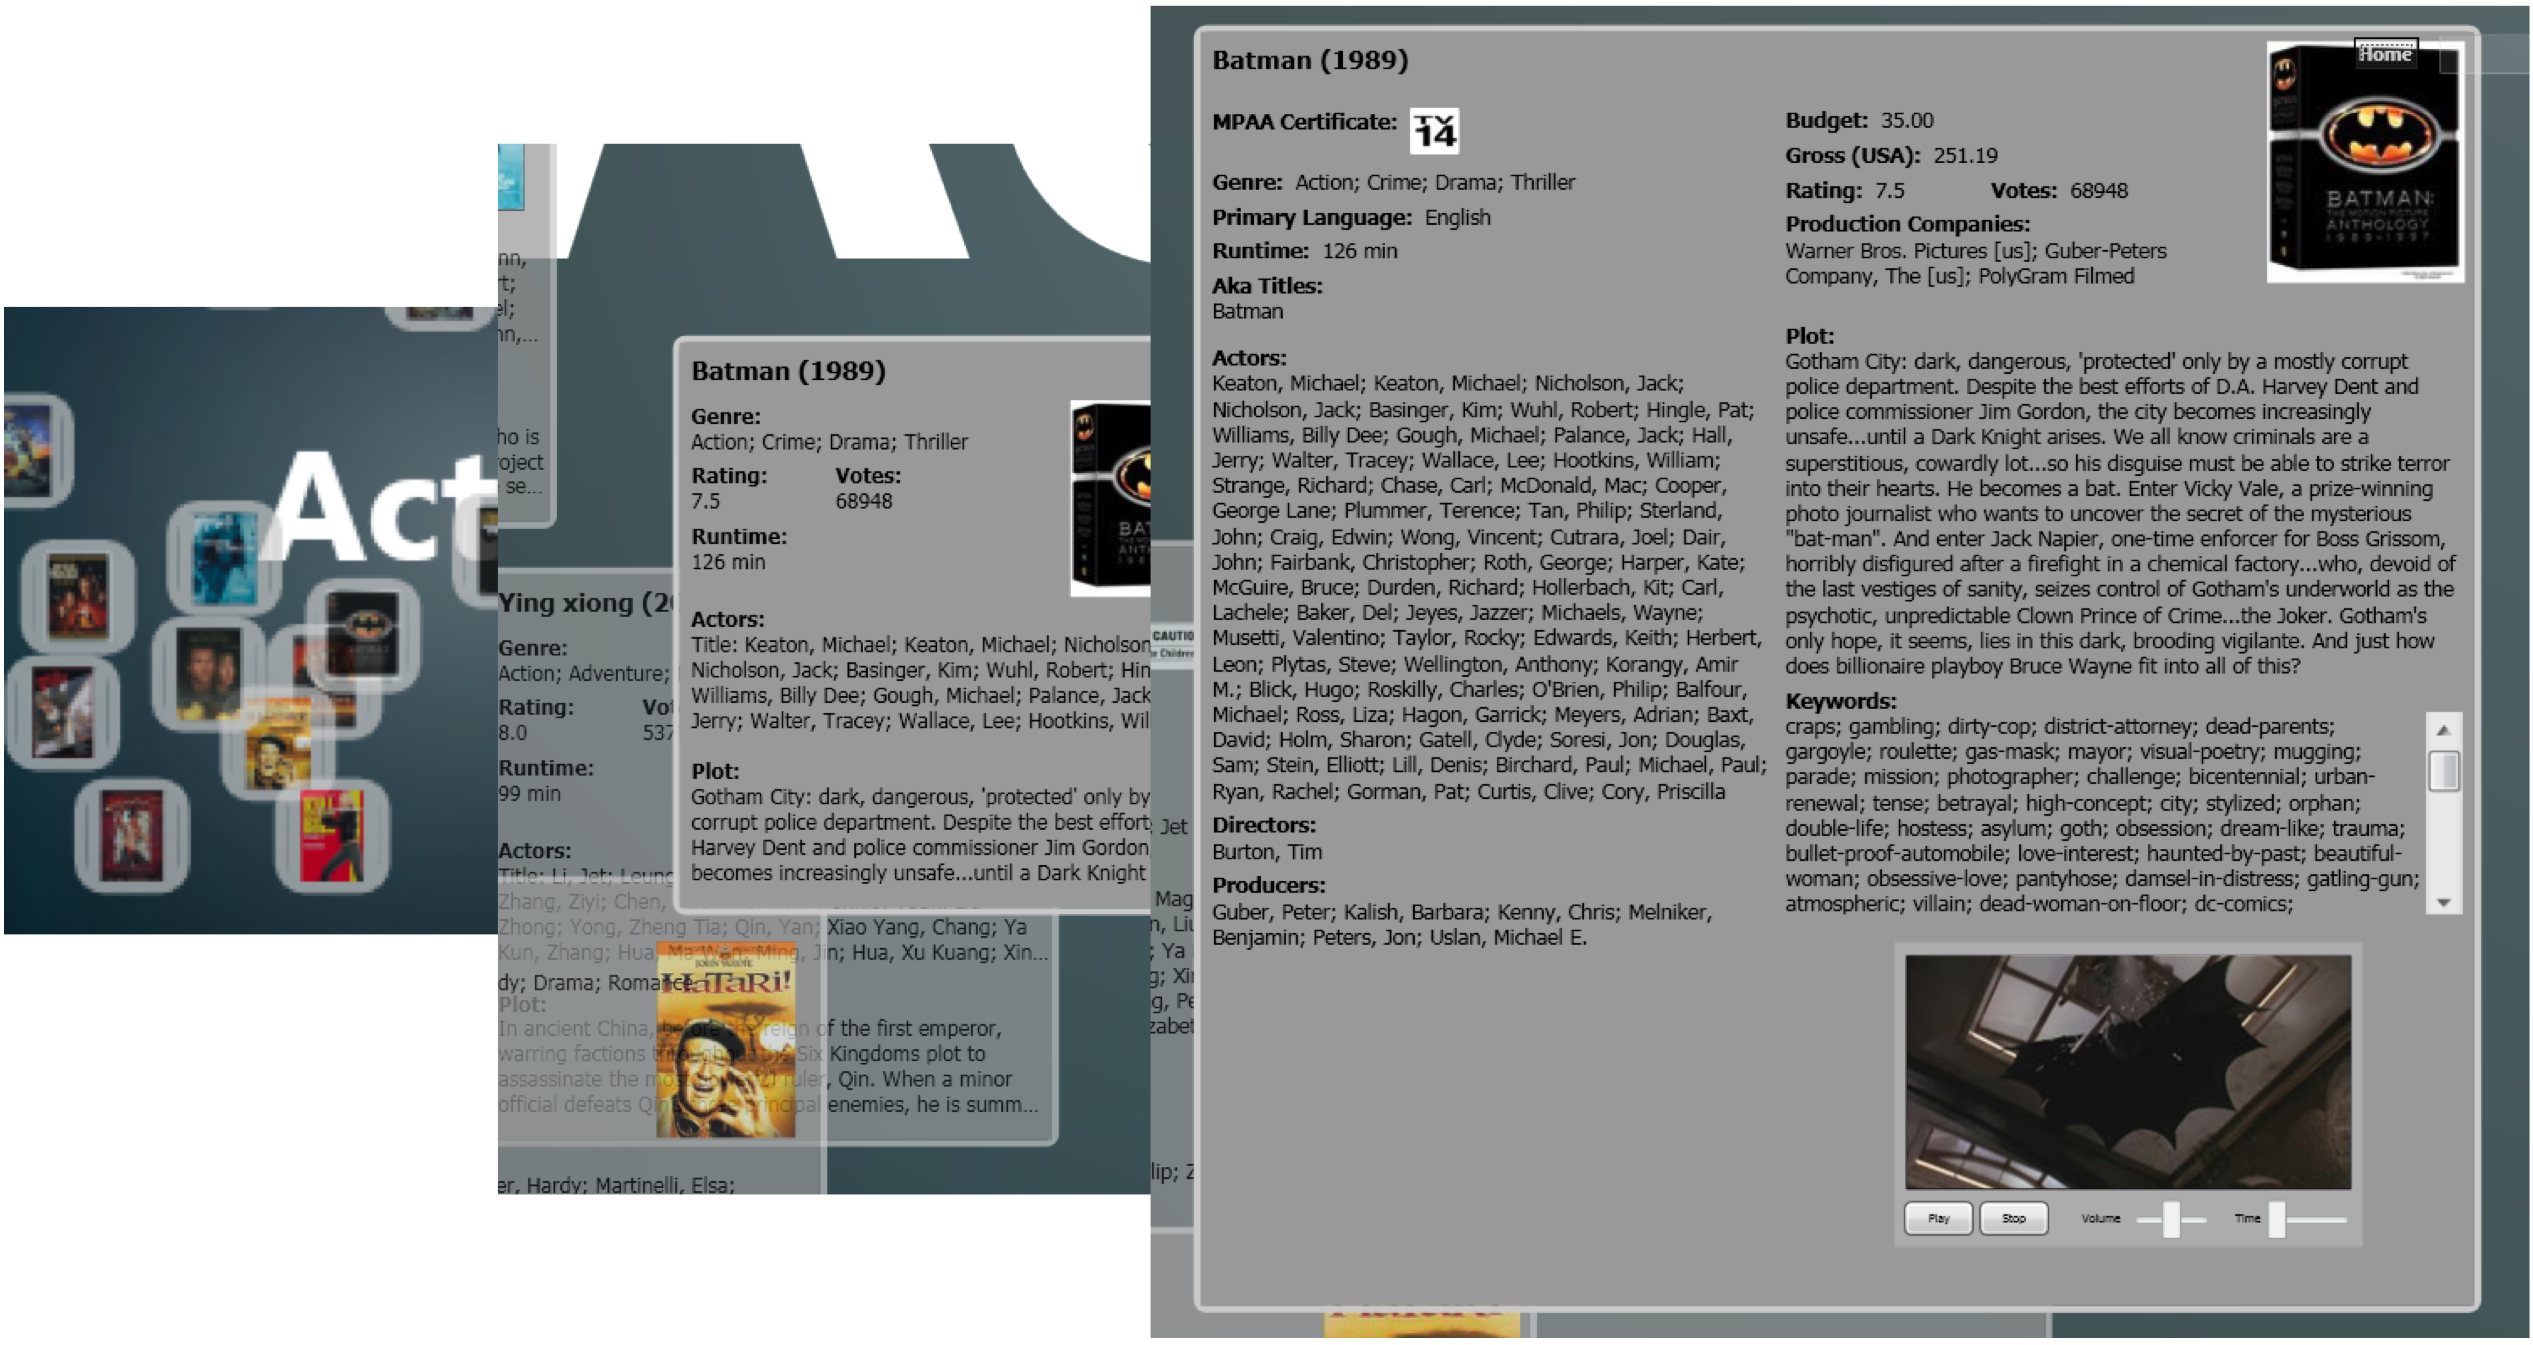
\includegraphics[width=\linewidth]{mediovis2.png}
 \caption{Ukážka sémantického zväčšenia\label{fig:semantic-zoom}}
\end{figure}

\section{Implementácie}

V tejto časti si popíšeme dve najpoužívanejšie implementácie ZUI, čo sú virtuálne plochy a počítačové mapy. Ďalej sa pozrieme na vôbec prvý prototyp tohto druhu rozhrania -- \textit{Pad} a jeho nasledovníka \textit{Pad++}. Stručne spomenieme ambiciózny projekt, ktorý mal používať len \textit{Zooming User Interface} na interakciu s používateľom -- \textit{Zoomworld}, a nakoniec aplikáciu \textit{Raskin}, ktorá kombinuje tradičné GUI a ZUI dokopy.

\subsection{Virtuálne plochy}
Jednou z najpoužívanejších a najrozšírenejších implementácií \textit{Zooming User Interface} sú virtuálne plochy, ktoré avšak ponúkajú len obmedzenú funkcionalitu oproti ostatným existujúcim riešeniam.

Pojem \uv{virtuálna plocha} označuje koncept, ktorý rozširuje správu okien v desktopových prostrediach, o možnosť umiestňovať okná do samostatných skupín, resp. na rôzne plochy. Tie dokážu koexistovať, avšak aktívna je vždy len jedna plocha. Teda ak používateľ pracuje s len s pár oknami, pričom má otvorené aj ďalšie, ktoré nepotrebuje, môže si nepotrebné okná premiestniť na samostatnú plochu, kde mu nebudú prekážať a môže sa tak sústrediť na prácu.

Podobnosť so ZUI nastáva pri zobrazení všetkých virtuálnych plôch zároveň. Používateľ teda získava prehľad o všetkých plochách a ich oknách súčasne. Pri tomto zobrazení má teda používateľ najlepšiu možnosť manipulovať s oknami (presun, zatvorenie), či samotnými plochami (pridávanie, odoberanie alebo zmena usporiadania).

Tento virtuálnych plôch vznikol, podobne ako celá WIMP paradigma, vo výskumnom stredisku Xerox PARC v roku 1986 pod názvom \textit{Rooms} \cite{rooms} a neskôr bol prevzatý aj do iných prostredí, kde zastáva neoddeliteľnú súčasť pri práci s oknami.

Táto funkcionalita je typická pre desktopové prostredia alebo správcov okien nachádzajúcich sa na unixových systémoch, ktoré obsahujú \textit{X Window System}. Medzi najznámejšie príklady, ktoré implementujú túto funkciu patria \textit{KWin} (prostredie \textit{KDE}), \textit{Metacity} (prostredie \textit{Gnome}), \textit{Compiz}, \textit{Fluxbox} a mnoho ďalších.

Iné operačné systémy nie sú výnimkou. \textit{Mac OS X} vyvíjaný spoločnosťou \textit{Apple} od verzie 10.5 ponúka totožnú funkciu pod názvom \textit{Spaces} (obr. \ref{fig:spaces}). Naproti tomu operačný systém \textit{Windows} od spoločnosti \textit{Microsoft} umožňuje používať funkciu len vďaka rôznym doplnkom, ktoré nie sú súčasťou samotného systému.

\begin{figure}
 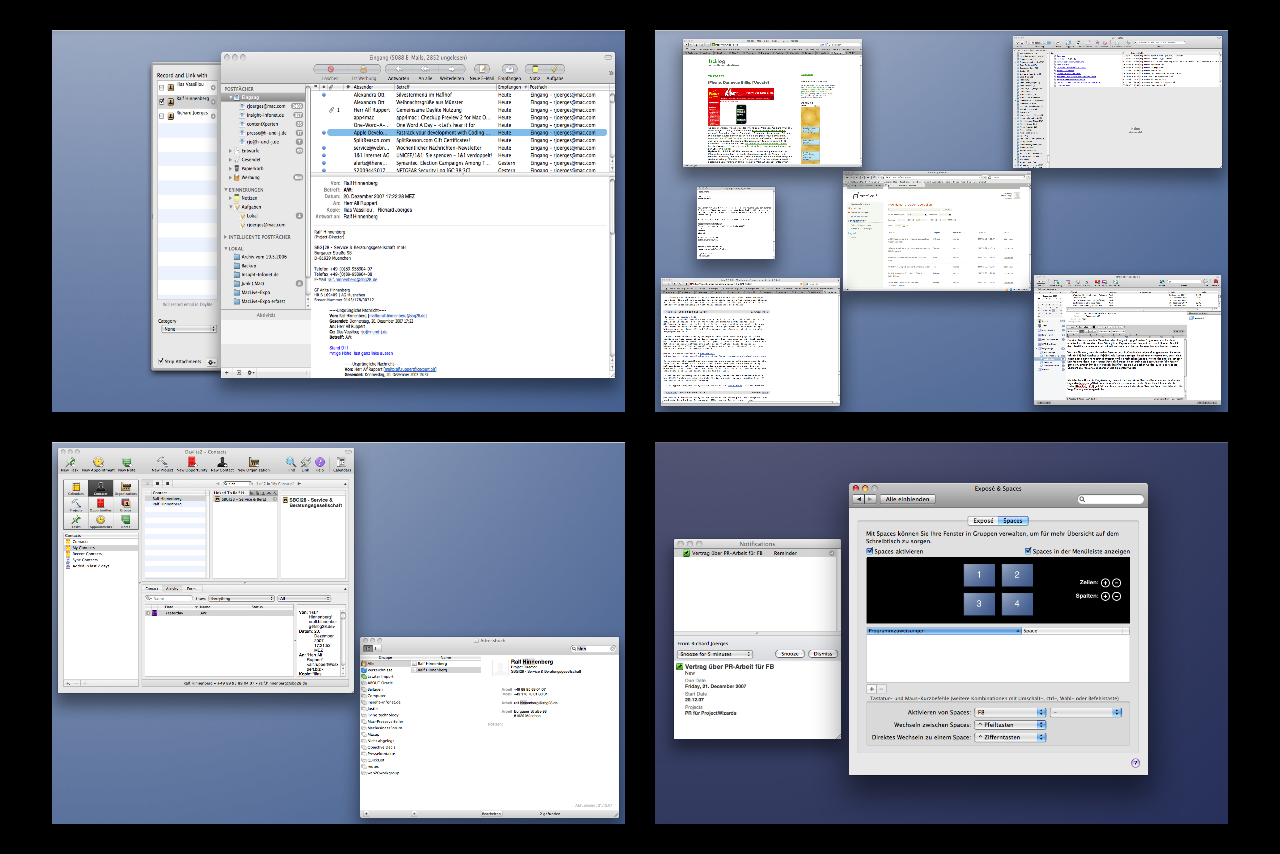
\includegraphics[width=\linewidth]{spaces}
 \caption{Spaces -- virtuálne plochy v Mac OS X\label{fig:spaces}}
\end{figure}

\subsection{Počítačové mapy}

Veľmi typické použitie \textit{Zooming User Interface} sú počítačové mapy. Aj napriek tomu, že sa nejedná o ZUI podľa definície, táto paradigma slúži na prezeranie máp veľmi dobre a práca s nimi sa stáva veľmi intuitívnou aj vďaka podobnosti s reálnym svetom. Hlavnými zástupcami počítačových máp sú produkty \textit{Maps} a \textit{Earth} od spoločnosti \textit{Google}, \textit{Bing Maps} od spoločnosti \textit{Microsoft}, \textit{Ovi Maps} od \textit{Nokie} alebo otvorené mapy \textit{OpenStreetMap}.

Najväčším obmedzením väčšiny počítačových máp oproti klasickým implementáciám ZUI, je používanie rôznych dát pre rôzne stupne priblíženia. Táto technika sa používa najmä pri satelitných fotografiách zemského povrchu, ale vektorové podklady nie sú výnimkou. Hlavným dôvodom pre toto obmedzenie je najmä šetrenie prostriedkami ako pamäť, disk, či pripojenie do Internetu. Dalo by sa tvrdiť, že táto vlastnosť je je akýmsi simulovaním sémantického priblíženia.

\subsection{Pad} \label{sec:pad}

\textit{Pad} \cite{pad} bola prvá implementácia \textit{Zooming User Interface} rozhrania na svete, za ktorou stoja Ken Perlin a David Fox. \textit{Pad} bol na svoju dobu (rok 1993) veľmi výnimočný projekt, ktorý išiel ďaleko za hranice tradičnej WIMP paradigmy. Okrem prvenstva medzi ZUI rozhraniami, priniesol aj veľmi revolučné myšlienky, ktoré postupne prichádzajú aj do používateľských rozhraní, ktoré denne používame.

Jednou z myšlienok, ktoré boli spolu s projektom \textit{Pad} predstavené je sémantické zväčšenie, ktoré je podrobnejšie popísané v časti~\ref{sec:semantic-zoom} \nameref{sec:semantic-zoom} na strane~\pageref{sec:semantic-zoom}. Ďalšou nemenej zaujímavou, avšak podstatne abstraktnejšou myšlienkou boli portály a tzv. \uv{portálové filtre}.

\subsubsection{Portály}

Portál označuje v tomto kontexte objekt, ktorý umožňuje presun k iným častiam plochy. Ako každý portál, aj tento má dva konce -- zdrojový a zobrazovací. Zdrojová časť sa umiestni na požadovanú časť plochy, ktorá má byť zobrazená cez portál. Zobrazovacia časť sa umiestni na požadovanú polohu, kde má byť zobrazená plocha zo zdroju. Veľmi vhodným umiestnením portálov by sme napríklad mohli simulovať fraktály.

\subsubsection{Portálové filtre}

Pojem portálové filtre označuje (nielen pri ZUI rozhraniach) spôsob vizualizácie istého zdrojového objektu iným objektom, ktorý modifikuje výzor zdrojového objektu podľa istých pravidiel. Najhlavnejším pravidlom je, že objekt, ktorý mení zdrojový objekt, musí \uv{rozumieť} dátam, ktoré poskytuje zdroj -- musia byť teda navzájom kompatibilné. Názorným príkladom môže byť tabuľka čísel, ktorá slúži ako zdroj dát. Ďalej máme portálový filter, ktorý rozpoznáva tabuľkové dáta a transformuje ich na koláčový graf. Ak presunieme tento portálový filter nad našu tabuľku, prekrytá časť tabuľky bude zobrazená ako graf. Ak portálový filter nemá zdroj dát, nemá žiadnu grafickú podobu, resp. nič nezobrazuje.

Tento koncept sa veľmi podobá na \textit{Model-View-Controller} \cite{mvc} architektúru, ktorá sa používa pri návrhu a implementácií aplikácií. \textit{Model} sa dá chápať ako zdroj dát, ktoré majú byť transformované a zobrazené cez \textit{view}. \textit{Controller} zabezpečuje prepojenie oboch častí, prípadne zmenu dát, ktoré sú obsiahnuté v modeli. Pri portálových filtroch je však situácia mierne odlišná. Všetky tri elementy majú grafickú podobu, čo pri MVC architektúre neplatí, kde len \textit{view} má takúto vlastnosť. Navyše, portálové filtre nemusia len zobrazovať dáta, ale môžu s nimi aj manipulovať, teda správať sa ako \textit{controller} alebo môžu spĺňať obe funkcie súčasne.

\subsection{Pad++} \label{sec:pad++}

Po úspechu s \textit{Pad} v oblasti používateľských rozhraní, Jim Hollan a Ben Bederson začali v roku 1994 vyvíjať nasledovníka -- \textit{Pad++} \cite{pad++1}. Tento projekt je najdlhšie trvajúcou iniciatívou o vytvorenie ZUI rozhrania, aj napriek tomu, že vývoj bol v roku 1998 oficiálne zastavený \cite{pad++2}. Počas svojej existencie, však posunul ZUI naozaj ďaleko, o čom svedčia Bedersonove ďalšie projekty \textit{Jazz} \cite{jazz} a \textit{Piccolo} \cite{piccolo} (neskôr premenované na \textit{Piccolo2D}), v ktorých možno nájsť veľa myšlienok z \textit{Pad++}.

\textit{Pad++} úspešne aplikovalo ZUI princíp na rôzne problémy, ktoré nemajú veľa spoločné. Aplikácia obsahovala prehliadač dokumentov s osnovou, kresliaci program, prehliadač obsahu disku, či dokonca prehliadač HTML stránok, ktorý je možné vidieť na obrázku~\ref{fig:pad++}.

\begin{figure}[ht]
 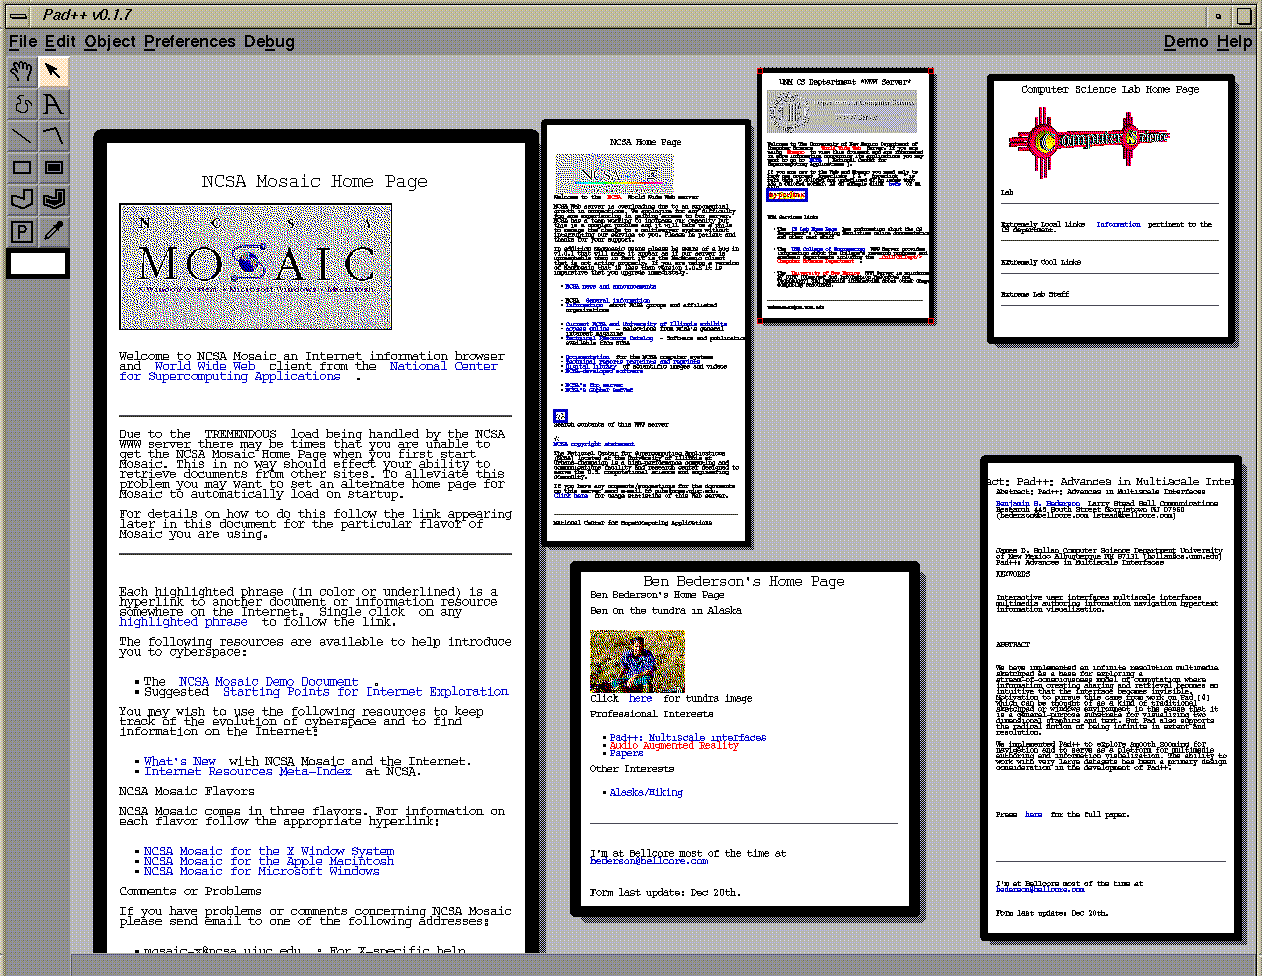
\includegraphics[width=\linewidth]{pad++}
 \caption{Pad++ -- prehliadač HTML stránok\label{fig:pad++}}
\end{figure}

\subsection{Zoomworld}

Jef Raskin, ktorý sa podieľal na vývoji počítaču \textit{Macintosh}, vo svojej knihe \textit{The Humane Interface} \cite{humane_interface} popisuje cestu za úplne prirodzeným používateľským rozhraním, ktoré by odstránilo dizajnové chyby WIMP paradigmy, viď. str.~\pageref{sec:wimp}. Raskin popisuje vtedajšie dostupné používateľské rozhrania ako bludiská, v ktorých sa používateľ často stráca pri dosiahnutí nejakého cieľa. Autor preto navrhuje vyriešiť tento problém \textit{oddialením} -- nazretím naň z výšky, odkiaľ vidieť štruktúru tohto bludiska a tým pádom sa mu vyhnúť a preletieť priamo k cieľu.

Raskin nazýva tento prístup \textit{Zooming Interface Paradigm} a konkrétny prípad takéhoto rozhrania popisuje v knihe ako \textit{ZoomWorld}. Autorovými slovami je popísaný takto:

\begin{quotation}
The ZIP [Zooming Interface Paradigm] described here is called ZoomWorld and is based on the idea that you have access to an infinite plane of information having infinite resolution. The plane is ZoomWorld. Everything you can access is displayed somewhere on ZoomWorld, whether it is on your computer, on a local network to which your computer is attached, or on a network of networks, such as the Internet.

To see more of ZoomWorld, you think of yourself as flying higher and higher above it. To look at a particular item, you dive down to it. ZoomWorld also has a content searching mechanism. The overall metaphor is one of flying, climbing to zoom out and diving to zoom in. You navigate both by flying above ZoomWorld and by doing content searches.
\end{quotation}

Vidíme, že \textit{ZoomWorld} popisuje ako nekonečnú plochu s nekonečným rozlíšením -- vieme sa priblížiť, či oddialiť bez akéhokoľvek obmedzenia. Toto je štandardná definícia ZUI rozhraní. Zaujímavejšie je však využitie takéhoto rozhrania -- na tomto plátne by bola zobrazená každá dostupná informácia, či už je na používateľovom počítači alebo na Internete. Touto myšlienkou sa \textit{ZoomWorld} líši od všetkých ostatných ZUI.

Z druhej časti časti citácie sa dozvedáme spôsob navigácie po ploche. Hlavným spôsobom pohybu je samozrejme priblíženie a oddialenie. \textit{ZoomWorld} avšak ponúka aj hľadanie obsahu na tejto nekonečnej ploche.

\textit{Zoomworld} bol len časťou vysnívaného používateľského prostredia, ktoré Raskin popísal. Snaha o implemetáciu tohto systému, pod názvom THE a neskôr \textit{Archy}, síce skončila, avšak myšlienky uvedené v knihe stále formujú budúce generácie používateľských rozhraní. Príkladom, kde sa uplatnili Raskinove nápady nesie jeho meno\dots

\subsection{Raskin}

\textit{Raskin} (obr.~\ref{fig:raskin}) je veľmi modernou kombináciou ZUI a tradičného WIMP rozhrania obsiahnutého v operačnom systéme Mac OS X. Štandardná pracovná plocha je nahradená zväčšovateľnou plochou, ktorá ponúka zobrazovanie dokumentov v plnom rozlíšení. Dokumenty je možné združovať do projektov, čím používateľ získava lepší prehľad nad stavom svojej práce. Spúšťanie aplikácií cez zástupcov ostalo v nezmenenej podobe -- aktivácia kliknutím na ikonu.

Zaujímavou funkciou je vloženie, alebo lepšie povedané, zapustenie okien do plochy, čo umožňuje asociovať otvorenú aplikáciu s rozpracovaným dokumentom. Týmto spôsobom je tiež možné prepínať sa medzi spustenými aplikáciami.

\begin{figure}[hb]
 \centering
 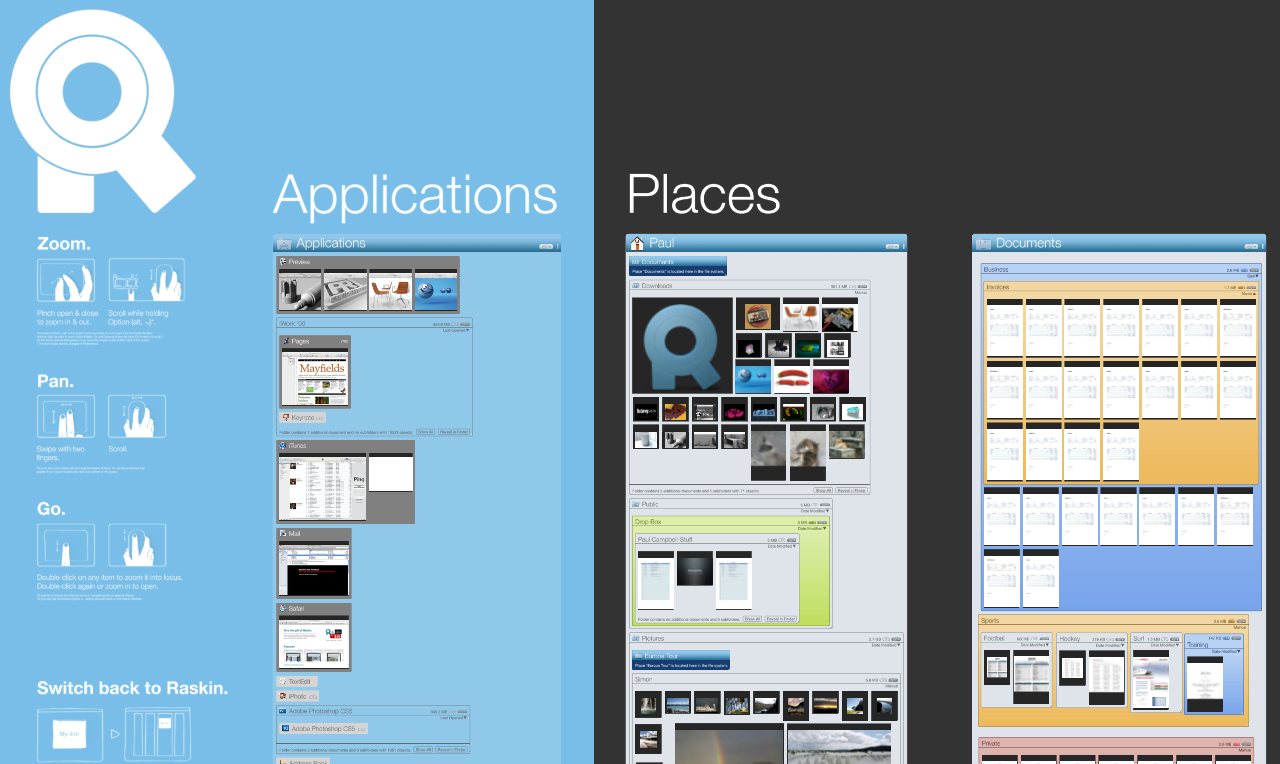
\includegraphics[width=\linewidth]{raskin}
 \caption{Raskin -- pohľad na časť plochy\label{fig:raskin}}
\end{figure}

\chapter{ZUI prezentačný softvér} \label{ch:zui_prezentacny_softver}

\section{Popis} \label{sec:zui-prezentation}

Ako vyplýva z názvu, ZUI prezentačný softvér využíva na prezentovanie informácií \textit{Zooming User Interface}, bližšie popísané v predchádzajúcej kapitole. Narozdiel od tradičných prezentačných programov, tento typ nevyužíva tzv. slajdy, opísané v časti \ref{sec:presentation_desc}. Namiesto toho sú jednotlivé informácie rozmiestnené na nekonečnej ploche a samotná prezentácia je zvyčajne realizovaná prechodom medzi vybratými časťami tejto plochy.

\subsection{Nelineárnosť prezentácie}

Veľkou výhodou oproti klasickým prezentačným programom je možnosť nelineárnej prezentácie. Ak by sme v tradičnom prezentačnom softvéri, ktorý používa slajdy, chceli poukázať na informáciu, ktorá sa nachádzala na začiatku prezentácie, museli by sme danú informáciu (alebo celý slajd) skopírovať na požadované miesto alebo sa pri samotnom akte prezentovania vrátiť na požadovaný slajd, čo by vyžadovalo zobraziť všetky informácie, ktoré boli spomenuté.

Pri ZUI prezentačnom softvéri môžeme uplatniť rovnakú stratégiu -- vrátiť sa po predefinovanej ceste k informácií, ktorú potrebujeme zobraziť. To však nie je optimálnym riešením. Lepším riešením je využiť zaujímavú vlastnosť ZUI prezentácií, ktorá nám umožňujú použiť jeden objekt v tejto ceste viackrát. Teda bez toho aby sme sa museli lineárne vracať, môžeme z aktuálneho bodu v ceste prejsť priamo na požadovanú informáciu. Hoci sa toto riešenie sa podobá na duplikáciu slajdu z tradičných prezentačných softvérov, k žiadnej duplikácií informácií nedochádza.

V predchádzajúcom príklade počítame s využitím už spomenutej informácie. Problém môže nastať ak sa prezentujúci nepočíta pri tvorbe prezentácie s takouto možnosťou. Ako sme spomenuli, pri prezentáciách, ktoré využívajú slajdy je nutné lineárne prejsť všetky informácie, ktoré sa nachádzajú medzi aktuálnym a požadovaným slajdom. Pri prezentácií, ktorá využíva ZUI je možné sa \uv{odkloniť} od cesty prezentácie a zobrazovať časti plochy podľa ľubovôle. Ak prezentujúci zobrazil všetky informácie, ktoré potreboval, môže pokračovať po ceste prezentácie.

\section{Existujúce riešenia}

Aj napriek tomu, že prvá zmienka použitia ZUI v prezentačnom softvéri je z roku 2001 \cite{counterpoint}, existuje len veľmi málo použiteľných riešení, ktoré sa sa stále vyvíjajú. V nasledujúcich odsekoch popíšeme štyri najvýznamnejšie implementácie tohto typu prezentačného softvéru.

\subsection{pptPlex}

Rozšírením \textit{pptPlex} do Microsoft PowerPoint (popísaným na strane~\pageref{sec:powerpoint}) verzie 2007, je možné dosiahnuť efektu podobného ZUI prezentačnému softvéru. Toto rozšírenie dodáva do aplikácie náhľad všetkých slajdov pre pohodlný výber toho, ktorý chceme zobraziť, bez toho aby sme museli lineárne prechádzať všetky slajdy medzi. Ďalšou možnosťou je zobraziť viacero slajdov na obrazovke naraz pre ich vzájomné porovnanie.

Z popisu zreteľne vidieť, že \textit{PowerPoint} s rozšírením \textit{pptPlex} neponúka rovnakú flexibilitu akú by mal ponúkať prezentačný softvér, ktorý by naplno využíval \textit{Zooming User Interface}. Projekt nezaznamenal od roku 2008 žiadnu aktivitu a teda je považovaný za mŕtvy.

\subsection{CounterPoint}

Iný prístup k rovnakému problému volí \textit{CounterPoint} \cite{counterpoint}, za ktorým stojí Lance Good a priekopník ZUI rozhraní Ben Bedereson. Hoci je \textit{CounterPoint} oveľa starší projekt ako \textit{pptPlex}, možnosti ktoré ponúka sú podstatne väčšie. Aj keď sa nejedná priamo o~doplnok do aplikácie Microsoft PowerPoint, stavia na ňom. Oproti \textit{pptPlex} umožňoval rozložiť slajdy na ploche, za ktorú je zodpovedný \textit{Jazz} (spomenutý v sekcií~\ref{sec:pad++} o~\nameref{sec:pad++}) a vytvoriť cestu, po ktorej ide prezentácia. Aj napriek tomu, že tento program ponúka lepšie využitie ZUI, stále sme obmedzení len na prechod medzi jednotlivými slajdami.

\subsection{Ahead}

\textit{Ahead} je webová aplikácia, naprogramovaná v \textit{Adobe Flash}, ktorá ponúka prezentovanie informácií na nekonečne veľkom plátne s využitím ZUI. Používate môže presúvať samotné objekty a nie len slajdy s informáciami ako pri predchádzajúcich dvoch príkladoch. Používateľ môže podobne ako pri aplikácií \textit{CounterPoint} určiť cestu, po ktorej pôjde prezentácia. \textit{Ahead} nie je určené len na prezentácie, ale môže byť využité aj ako web stránka, virtuálne múzeum, myšlienková mapa, či iné.

Hlavnou nevýhodou pri prezentovaní s \textit{Ahead} je animácia prechodu. Priblíženie a posunutie sú lineárne interpolované, čo nevytvára dobrý dojem zo samotnej prezentácie (viď. odsek~\nameref{sec:linear-interpolation} na strane~\pageref{sec:linear-interpolation}).

Vidíme, že doteraz žiadna z menovaných aplikácií nevyužíva naplno možnosti, ktoré by koncept ZUI prezentačného softvéru ponúkal.

\subsection{Prezi} \label{sec:prezi}

\textit{Prezi} je doteraz najlepšou voľbou na vytváranie prezentácií využívajúcich \textit{Zooming User Interface}. Ponúka všetky vlastnosti, ktoré mali už spomínané aplikácie a pridáva ešte mnoho ďalších inovatívnych prvkov.

\subsubsection{ZUI menu}

Veľmi zaujímavo je riešené hlavné menu aplikácie, viď. obrázok~\ref{fig:prezi-bubblemenu}, ktoré ako celá aplikácia využíva ZUI. Jednotlivé funkcie sú zobrazené ako kruhy rôznych veľkostí s textovým a niektoré aj grafickým popisom akcie. Veľkosť kruhu závisí od hierarchie funkcií, kde menej podstatnejšie funkcie majú menšiu veľkosť a opačne. Pri zvolení istej funkcie sa celá sústava kruhov priblíži, tak aby požadovaná skupina funkcií zaberala čo najväčšiu možnú plochu a ostatné funkcie boli stále prístupné. Vďaka priblíženiu sa odhalia funkcie, ktorých funkcia nebola predtým rozoznateľná kvôli ich veľkosti.

\subsubsection{Zebra}

Lineárne transformácie objektov na ploche, sú v \textit{Prezi} implementované netradičnou cestou. V aplikáciách, kde je vyžadovaná podobná funkcionalita, sa zvyčajne okolo aktívneho objektu zobrazí orámovanie, ktoré má aktívne rohy. Ťahaním týchto aktívnych rohov sa aktivuje uniformné škálovanie. Body, ktoré ležia na spojniciach rohov slúžia na neuniformné škálovanie. Translácia samotného objektu je aplikovaná jednoduchým ťahaním a pustením. Na rotáciu sú zvyčajne vyhradené dva body. Ťahaním jedného prevádzame samotnú rotáciu a druhý určuje stred otáčania.

Naproti tomu, v \textit{Prezi} nič podobné nenájdeme. Všetky tri transformácie sú spojené do jedného ovládacieho prvku, ktorý sa volá \textit{Zebra}. Tento prvok sa skladá z troch sústredných kruhov, z ktorých každý predstavuje inú transformáciu. Pri ťahaní najvnútornejšieho kruhu posúvame aktívnym objektom, pri ťahaní vnútorného kruhu uniformne škálujeme objekt a pri ťahaní vonkajšieho kruhu meníme objektu natočenie.

Zebru je možné vidieť v strede obrázku~\ref{fig:prezi-ui} prekrývajúc nápis \uv{Hello World!}.

\begin{figure}
  \centering
  \subfloat[Hlavné menu]{\label{fig:prezi-bubblemenu}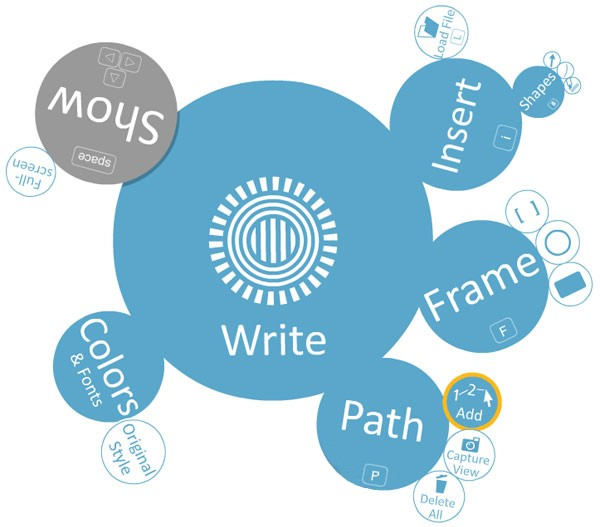
\includegraphics[width=0.45\textwidth]{prezi-bubblemenu.jpeg}}                
  \subfloat[Základné zobrazenie]{\label{fig:prezi-ui}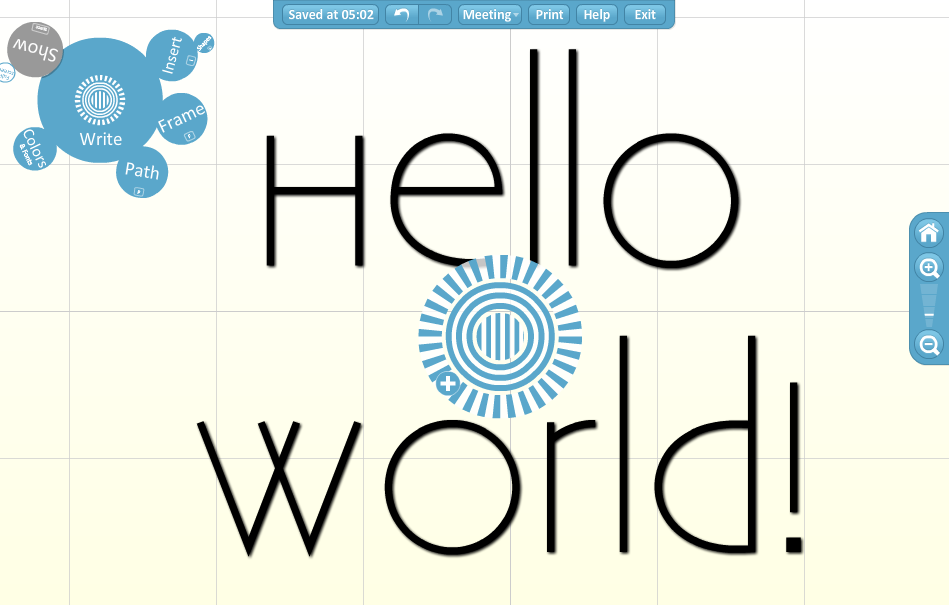
\includegraphics[width=0.55\textwidth]{prezi-ui.png}}
  \caption{Prezi}
  \label{fig:prezi}
\end{figure}

\subsubsection{Prvky na ploche}

Okrem štandardných prvkov ako text, obrázok, či video vieme do prezentácie vkladať aj iné objekty, ktoré spríjemňujú výsledný dojem z prezentácie. Najhlavnejšími sú:

\begin{itemize}
 \item zátvorky, kruh, obdĺžnik
 \item šípky, čiary
 \item kreslenie, zvýraznenie
\end{itemize}

Prvá kategória je určená na združovanie rôznych objektov do skupín, aby mohli byť zobrazené pri prezentácií ako celok a nie len po jednom. Okrem týchto troch objektov existuje ešte štvrtý, ktorý vykonáva rovnakú funkciu, ale nemá grafickú podobu.

Šípky a čiary pomáhajú zobraziť vzťah medzi jednotlivými objektami, či poslúžiť pri referencií na iné objekty.

Kreslením môžeme načrtnúť nejaký tvar alebo obrázok, ktorý nemáme k dispozícií a zvýrazňovačom zdôrazniť nejaký významný text alebo časť obrázku.  

\subsubsection{Zmena štýlu}

\textit{Prezi} disponuje veľmi užitočnou funkciou, ktorá je však určená len pre pokročilých používateľov. Tým je zmena grafického výzoru prvkov na ploche, či dokonca samotnej plochy, pomocou kaskádových štýlov, angl. \textit{Cascading Stylesheet} (CSS). Táto funkcionalita dáva používateľovi neobmedzenú možnosť prispôsobiť si prezentáciu do najmenších detailov. Pre používateľov, ktorý neovládajú CSS sú predpripravené témy, medzi ktorými môžu jednoducho prepínať.

\subsubsection{Nevýhody}

Hoci je \textit{Prezi} v kategórií ZUI prezentačných programov jednoznačne najlepšia voľba, má určité nevýhody, ktoré škodia celkovému dojmu z aplikácie:

\begin{itemize}
 \item webová aplikácia
 \item platená \textit{Pro} licencia
 \item implementované v \textit{Adobe Flash}
 \item proprietárny softvér
 \item povinné zverejnenie prezentácií s normálnym používateľským kontom
\end{itemize}

Prvé bod sa dá vnímať dvojako. Na jednej strane to môžeme vnímať ako výhodu, z~dôvodu dostupnosti z~celého sveta, ale aj ako nevýhodu ak práve nemáme dostupné pripojenie k  Internetu. Táto nevýhoda je minimalizovaná možnosťou stiahnuť si natívnu aplikáciu, ktorá je avšak dostupná len platiacim zákazníkom s \textit{Pro} licenciou, spomenutou v druhom bode.

Obe tieto aplikácie -- webová aj natívna, sú však naprogramované v \textit{Adobe Flash}, ktorý má svoje obmedzenia. Najväčšou nevýhodou použitia tejto technológie je nutnosť mať zásuvný modul do webového prehliadača, ktorý však znižuje jeho stabilitu. Ďalšou negatívnou vlastnosťou je absencia hardvérovo-urýchľovaného vykresľovania na desktopoch.

V oboch spomínaných prípadoch sa jedná o proprietárny softvér, teda o softvér s uzavretým zdrojovým kódom. Avšak v spojení s prvými dvoma negatívami, táto vlastnosť vytvára možnosť pre finančný zisk pre spoločnosť, ktorá zastrešuje vývoj aplikácie.

Poslednou nevýhodou je povinné zverejňovanie vytvorených prezentácií na webovej stránke aplikácie. Toto obmedzenie sa však netýka študentov s edukačnou licenciou a platiacich zákazníkov.

\chapter{Návrh práce} \label{ch:navrh}

V nasledujúcej kapitole popíšeme návrh aplikácie určenej na tvorbu a zobrazovanie prezentácií využívajúcich \textit{Zooming User Interface}.

\section{Editačná časť}

Podstatnou, aj keď nie vždy nutnou vlastnosťou prezentačného softvéru, je schopnosť vytvárať prezentácie. V prípade ZUI prezentačného programu je to nasledovné:

\begin{itemize}
 \item pridávanie a odoberanie prvkov z plochy
 \item zmena ich vlastností (veľkosť, pozícia, natočenie, \dots)
 \item vytvorenie cesty prezentácie
 \item navigácia po ploche
\end{itemize}

Aby bola zaistená prvá podmienka, používateľ bude mať k dispozícií objekty, z ktorých každý jeden bude predstavovať istý typ objektu, či už je to textový alebo grafický prvok. Ťahaním tejto reprezentácie prvku na plochu sa vytvorí inštancia požadovaného objektu, ktorý môže byť ďalej upravovaný. Odobratie prvku z plochy bude aplikovateľné presne opačným postupom -- ťahaním objektu z plochy na jeho reprezentáciu.

Zmena veľkosti, pozície a natočenia objektu na ploche, bude možné meniť pomocou ťahania aktívnych rohov každého objektu. Tento prístup používajú takmer všetky grafické programy a používateľ sa tak nebude musieť učiť novým návykom.

Na vytvorenie cesty prezentácie, bude potrebné sa prepnúť do špeciálneho módu. Keď bude tento mód aktívny, výber nejakého objektu, bude mať za následok pridanie tohto objektu do cesty. Zároveň sa bude zobrazovať aj samotná cesta v podobe spojených úsečiek, ktoré budú mať krajné body v stredoch objektov, ktoré sú obsiahnuté v ceste.

Na to aby sme vedeli previesť všetky popísané akcie tak ako chceme, musíme sa vedieť pohybovať po ploche. To pri \textit{Zooming User Interface} docielime priblížením, resp. oddialením a posunom plochy. Zmena priblíženia bude možná cez tlačidlá v rozhraní, prípadne rolovaním kolieska myši. Posun bude možný ťahaním prázdneho miesta plochy.

\subsection{Prvky}

Dvomi základnými prvkami, ktoré sa budú dať pridať na plochu sú text a obrázky. Aj napriek tomu, že konkurenčné programy ako napr. \textit{Prezi}, ponúkajú väčšie množstvo prvkov, naša aplikácia bude obsahovať systém rozšírení, vďaka ktorému bude možné neskôr doplniť do aplikácie ďalšie prvky.

\section{Prezentačná časť}

Pri prezentačnom softvéri, ktorý využíva zobrazovanie informácií pomocou \textit{Zooming User Interface} je veľmi dôležitá plynulosť zobrazovaného obsahu, tak aby divák nestratil prehľad nad zobrazovanými informáciami. Preto je potrebné venovať veľkú pozornosť pri návrhu prezentačnej časti.

\subsection{Cesta prezentácie}

Ako sme spomenuli v predchádzajúcich častiach, ZUI prezentačný softvér môže, ale nemusí používať pri samotnej prezentácií cestu, po ktorej sa prezentácia uberá. Rozhodli sme sa, že naša aplikácia sa bude striktne držať cesty. Jediná možnosť kedy bude možné z tejto cesty zísť je opustenie prezentačného módu.

\subsection{Animácia prechodu}

Ako už bolo spomenuté, používateľ, resp. divák, sa musí orientovať na zobrazovanej ploche, tak aby nestratil prehľad nad zobrazovanými informáciami. To dosiahneme animáciou, ktorá zjemní prechod medzi jednotlivými objektami. Keďže zobrazované objekty sa môžu líšiť rozmermi, polohou a otočením, je nutné zabezpečiť aby animácia brala do úvahy všetky tri parametre.

Naša stratégia bola nasledovná: vždy keď sme objavili nový model akým by mohla animácia poskytovať dostatočný dojem, implementovali sme prototyp, ktorý sa správal podľa modelu a následne sme ho otestovali. Ak vyhodnotenie testovania neprinieslo požadované výsledky, proces sme zopakovali.

\subsubsection{Lineárna interpolácia} \label{sec:linear-interpolation}
Naivným prístupom by sme dospeli k animácií, ktorá lineárne interpoluje všetky hodnoty medzi dvoma známymi bodmi. Aj napriek jednoduchosti implementácie by neponúkala dostatočné výsledky. Animácia by sa z pohľadu používateľa dala popísať takto:

\begin{enumerate}
 \item pozeráme sa na prvý objekt, animácia začne
 \item prvý objekt zmizne z výhľadu
 \item náhodné objekty \uv{prebehnú} obrazovkou
 \item zobrazí sa druhý objekt, animácia skončí
\end{enumerate}

Z popisu animácie už tušíme, že výsledný dojem nebude pre diváka príjemný a preto treba skúsime nejaké lepšie riešenie.

\subsubsection{Easing curve}

Možným vylepšením môže byť použitie tzv. \textit{easing curve}, teda \uv{uvoľňovacej krivky}. Tá funguje podobne ako lineárna interpolácia, avšak s jedným rozdielom. Ak by sme chceli animovať presun objektu z bodu $A$ do bodu $B$, v oboch prípadoch by sme dostali trajektóriu pre objekt priamku z $A$ do $B$. Pri lineárnej animácií by mal objekt konštantnú rýchlosť, avšak pri použití \textit{easing curve} by mohol objekt najskôr zrýchľovať a následne spomaľovať -- vieme ovplyvňovať beh času nejakou funkciou.

Na prvý pohľad sa to nezdá ako výrazné zlepšenie, avšak toto riešenie poskytuje lepší výsledný dojem z animácie. V reálnom svete sa objekty nezačnú okamžite hýbať alebo okamžite zastaviť, preto na diváka pôsobí animácia organickejšie.

Aj napriek miernemu zlepšeniu, prototyp tejto animácie, ktorý sme testovali, stále trpel rovnakými problémami ako jednoduchá lineárna interpolácia -- používateľ stráca prehľad kde sa objekty nachádzajú, aká je medzi nimi vzdialenosť a pod.

\subsubsection{Oddialenie, posun, priblíženie}

Možným riešením straty používateľovho prehľadu nad objektami, by mohla byť nasledovná stratégia:

\begin{enumerate}
 \item oddialenie sa od prvého objektu, aby boli oba objekty viditeľné
 \item presun nad druhý objekt
 \item priblíženie sa k druhému objektu
\end{enumerate}

Prvým bodom animácie docielime, že používateľ vidí vzájomnú polohu oboch objektov, čím sa dosiahne lepší prehľad medzi súvisom oboch objektov. Vidíme, že pri tomto riešení často využívame vlastnosť \textit{Zooming User Interface} rozhraní -- zmenu priblíženia. Obe tieto skutočnosti naznačujú, že ideme správnym smerom.

Doposiaľ sme brali do úvahy len mieru priblíženia a posun plochy -- nespomenuli sme kde by sa mala odohrávať rotácia. Existujú tri použiteľné alternatívy kedy animovať rotáciu:

\begin{itemize}
 \item počas oddialenia, resp. priblíženia
 \item počas presunu z jedného na druhý objekt
 \item počas celej animácie
\end{itemize}

Prvá možnosť predstavuje nasledovný scenár: pohľad sa z uhlu rovnému zápornej hodnote otočenia prvého objektu zmení animáciou na nulový uhol, nasleduje posun kedy sa uhol nemení a pokračuje obdobne ako na začiatku celej animácie. Pri vyhodnotení prototypu animácie tohto druhu sme neboli spokojní s výsledkom. Rotácia bola rozkúskovaná, čo vytváralo dojem nejednotnosti.

V druhej alternatíve sa rotácia pohľadu mení pri presune z objektu na objekt. Pri testovaní tejto možnosti bol výsledok lepší ako pri predchádzajúcom postupe, avšak stále sa animácia javila ako nekonzistentná, preto sme skúsili poslednú možnosť.

Posledným dostupným riešením je meniť rotáciu počas celej dĺžky animácie ako sme robili pri lineárnej interpolácií. Aj napriek prvotnému skepticizmu, rotácia s touto stratégiou  dosahovala dosiaľ najlepšie výsledky a boli sme rozhodnutí zvoliť tento typ animácie.

\subsubsection{Plynulá a efektívna animácia}

Hoci sme sa rozhodli použiť vyššie popísanú animáciu, neboli sme úplne spokojní s~výsledkom -- animácia nebola plynulá. Prezi, popísané v sekcií~\ref{sec:prezi} na strane~\pageref{sec:prezi}, poskytuje omnoho príjemnejší a plynulejší prechod medzi dvoma objektami. Preto sme sa snažili zistiť ako je ich animácia definovaná. V \cite{prezi} sa nám podarilo nájsť referenciu na článok s názvom \textit{Smooth and Efficient Zooming and Panning} \cite{wijk1}, kde autor zavádza definíciu pre plynulú a efektívnu animáciu rovnakého typu akú potrebujeme.

\begin{figure}
 \centering
 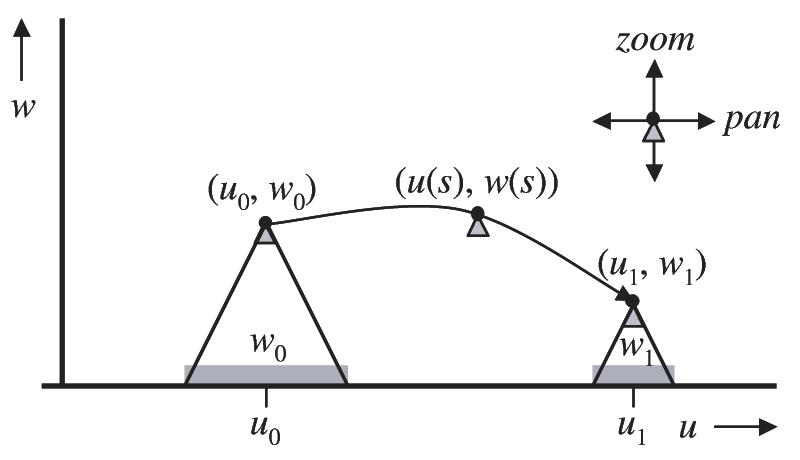
\includegraphics[width=0.75\linewidth]{uw-diagram.jpeg}
 \caption{Ukážka $u,w$ diagramu\label{fig:uw-diagram}}
\end{figure}

Autori na lepšie znázornenie priblíženia a posunu v animácií používajú tzv. \textit{$u,w$ diagramy} \cite{uw-diagrams} (ukážka na obrázku~\ref{fig:uw-diagram}), kde $u$ vyjadruje mieru posunutia a $w$ mieru priblíženia, resp. oddialenia. Body $(u_0,w_0)$ a $(u_1,w_1)$ sa dajú chápať ako umiestnenia kamery, ktorá v prvom bode zachytáva objekt s veľkosťou $w_0$, pozíciou $u1$ a obdobne pre druhý bod. Trajektóriu pre kameru definujú funkcie $u(s)$ a $w(s)$, kde $s \in [0,S]$ vyjadruje čas, ak rýchlosť animácie je jednotková.

Podobne ako my, autori najskôr skúsili stratégiu \uv{oddialenie, posun, priblíženie}, z~ktorého neskôr odvodili optimálnu cestu kamery ponad plochu. Tá sa nachádza na geodetickej  krivke v $u,w$ diagrame a má jeden nastaviteľný parameter $\rho$. Ten ovplyvňuje mieru priblíženia -- ak je $\rho = 1$ trajektória kamery leží na polkružnici. Ak je parameter väčší, $w$ bude mať väčšiu hodnotu, teda plocha sa oddiali viac. Ak je parameter menší, plocha sa oddiali menej. Článok uvádza optimálnu hodnotu parametru $\rho$, zistenú používateľskými testami, rovnú $\sqrt{2}$.

Pri implementácií prototypu sme avšak narazili na nedostatok popisovaného prístupu -- model nepočíta s rotáciou objektov. Skúsili sme popisovanú stratégiu zlúčiť s lineárnou interpoláciou, avšak výsledok nebol konštantne uspokojivý. Dôvodom bolo nezapočítanie času potrebného na rotáciu do koncovej hodnoty animácie $S$. Ak bola vzdialenosť dvoch objektov minimálna, avšak ich rotácia sa výrazne líšila, výsledný čas animácie bol veľmi krátky, teda rotácia musela prebehnúť rýchlo. Vidíme, že rýchlosť rotácie nebude vždy stála, s čím sme neboli spokojní.

\subsubsection{Model pre plynulé zobrazovanie a navigáciu v 2D priestoroch} \label{sec:animation}

Autori predchádzajúceho článku pokračovali v odvodzovaní definície pre plynulú a efektívnu animáciu v článku \textit{A Model for Smooth Viewing and Navigation of Large 2D Information Spaces} \cite{wijk2}. Tam používajú rovnaký princíp odvodzovania pre ďalšie lineárne transformácie ako napr. rotáciu, či neuniformné škálovanie. Správne sme predpokladali, že na dosiahnutie konštantnej rýchlosti rotácie potrebujeme zahrnúť rotáciu oboch objektov do $S$.

Nasledujúce rovnice vyjadrujú trajektóriu kamery, ktorú implementujeme v aplikácií na animáciu prechodu z jedného objektu na druhý.
\begin{subequations}
\label{eq:animation}
\begin{align}
\alpha(s) &= (\alpha_1 - \alpha_0) s / S + \alpha_0 \label{eq:alpha}\\
u(s) &= \frac{w_0}{\rho^2} \cosh r_0 \tanh ((r_1 - r_0) s/S + r_0) - \frac{w_0}{\rho^2} \sinh r_0 + u_0\\
w(s) &= \frac{w_0 \cosh r_0}{\cosh \left(\left(r_1 - r_0\right) s/S + r_0\right)}\\
S &= \sqrt{\frac{(\alpha_1 - \alpha_0)^2}{\mu^2} + \frac{(r_1 - r_0)^2}{\rho^2}} \label{eq:S}\\
r_i &= \ln \left(-b_i + \sqrt{b_1^2 + 1}\right), i = 0, 1 \\
b_i &= \frac{w_1^2 - w_0^2 + (-1)^i \rho^4 (u_1 - u_0)^2}{2 w_i \rho^2 (u_1 - u_0)}, i = 0, 1
\end{align}
\end{subequations}

Ako vidíme, z rovníc~\eqref{eq:animation}, tak vzťah na vyjadrenie rotácie $\alpha$ \eqref{eq:alpha} je lineárna interpolácia, ktorú sme skúšali aj predtým. Rozdiel je v zahrnutí $\alpha_0$ a $\alpha_1$ v rovnici~\eqref{eq:S}. Pozorný čitateľ si všimneme, že pribudol nový parameter $\mu$, ktorý ovplyvňuje rýchlosť rotácie a tým pádom aj celé trvanie animácie. Autori článku opäť empiricky zistili, že optimálna hodnota parametra $\mu$ je rovná približne $\sqrt{6}$.

\section{Architektúra}

Najdôležitejšou časťou prezentačného programu je zobrazovacia vrstva. Esenciálna nie je len pri samotnom čine prezentovania informácií, ale aj pri vytváraní prezentácie -- rozmiestňovaniu objektov po ploche. Architektúra prezentačnej vrstvy, ktorú možno vidieť na obrázku \ref{fig:schema}, sa skladá z troch hlavných komponentov: \texttt{ZuiView}, \texttt{ZuiItem} a \texttt{ZuiHelper}.

\begin{figure}
 \centering
 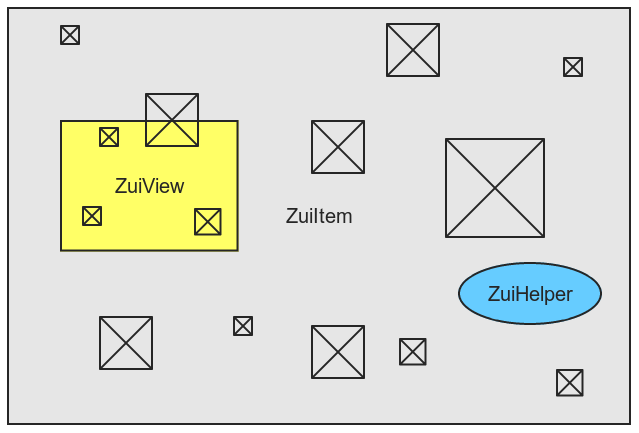
\includegraphics[width=0.75\linewidth]{architektura}
 \caption{Schéma architektúry prezentačnej vrstvy\label{fig:schema}}
\end{figure}

\subsection{ZuiView}
\texttt{ZuiView} je vizuálny komponent, s ktorým sa priamo interaguje, resp. ako jediný sa vkladá do používateľského rozhrania. Poskytuje vysokoúrovňové funkcie ako napr. začať a ukončiť prezentáciu, pridávanie objektov na plochu, priblíženie, či oddialenie, atď.

\texttt{ZuiView} nevykonáva samotné akcie, ale manažuje nízkoúrovňový komponent \texttt{ZuiItem}, ktorý zabezpečujú požadovanú funkcionalitu. Dôvodom pre takéto \uv{obalenie} funkčného komponentu je niekoľko.

Prvým dôvodom je nutnosť orezania zobrazovaného výstupu (angl. \textit{clipping}), ktorý produkuje \texttt{ZuiItem}. Aj napriek tomu, že \texttt{ZuiView} bude zobrazený vždy na celé okno aplikácie (teda nie je nutnosť výstup orezávať), počítame so širším využitím tohto komponentu (napr. v iných aplikáciách). Preto je dobré počítať s takouto možnosťou a obaliť \texttt{ZuiItem} do \texttt{ZuiView}.

\subsection{ZuiItem}

Ako je vidieť na schéme architektúry (obr.~\ref{fig:schema}), \texttt{ZuiItem} nie je obyčajný vizuálny komponent ako \texttt{ZuiView}. Aj napriek tomu, že technicky sa jedná o vizuálny prvok (existuje v súradnicovom systéme), tak nemá žiadnu grafickú podobu. Tento objekt slúži ako samotná virtuálna plocha -- rodič pre všetky ostatné elementy prezentácie.

\texttt{ZuiView}, ktorý disponuje zmenou priblíženia je implementovaný v tomto komponente ako jednoduché škálovanie celého objektu, vrátane jeho detí. Rovnakým spôsobom sa prevádza rotácia a translácia.

Veľmi dôležitou podmienkou pri aplikovaní rotácie a škálovania je nutnosť udržiavať stred otáčania, resp. počiatočný bod škálovania, v strede komponentu \texttt{ZuiView}.

\subsection{ZuiHelper}

\texttt{ZuiHelper} je špeciálny objekt, ktorý nemá grafickú podobu a iba poskytuje informácie o lineárnych transformáciách pre \texttt{ZuiItem}. Ak je nutné pri prezentácií vykonať animáciu prechodu z jedného na druhý objekt, tento komponent vypočíta trajektóriu kamery ponad plochu podľa rovníc popísaných v časti \nameref{sec:animation} na strane~\pageref{sec:animation}.

Tento komponent má vlastný časovač, ktorý riadi popísanú animáciu. Ak je vyžiadaný prechod na ďalší objekt počas trvania animácie, \texttt{ZuiHelper} automaticky vypočíta novú trajektóriu z aktuálneho pohľadu na cieľový objekt.

\section{Používateľské rozhranie}

Hoci na prezentáciu bude použité ZUI používateľské rozhranie, ostatné prvky aplikácie budú využívať tradičné rozhranie. Aj napriek tomu, že myšlienka ZUI menu v Prezi, je veľmi zaujímavá, pre ciele tejto práce bohužiaľ irelevantná.

Základným východiskom pri návrhu používateľského rozhrania, je snaha čo najviac využiť Fittsov zákov \cite{fitts}. Dôsledkom tohto rozhodnutia je nutnosť zabrať aplikáciou celú obrazovku, aby okraje a rohy boli v aplikácií prístupné. Do oblastí, ktoré sú podľa tohto zákona najlepšie dosiahnuteľné, umiestnime panely s akciami. Tieto panely však budú maximálny možný čas skryté, aby neprekážali pri navigácií po ploche. Prístupné budú len po aktivácií, čo v našom prípade znamená presun kurzoru na hranu, či do rohu obrazovky.

Na obrázku \ref{fig:ui} môžeme vidieť návrh rozhrania pri tvorbe prezentácie (obr.~\ref{fig:editacia}) a pri aktívnom prezentačnom móde (obr.~\ref{fig:prezentacia}). Ako vidíme, používateľské rozhranie je naozaj minimálne. Je však pravdepodobné, že pri implementácií nastanú nejaké zmeny, ktoré však teraz nezohrávajú veľkú úlohu.

Pri tvorbe prezentácie máme k dispozícií hlavné menu a paletu komponentov, ktoré môžeme využiť. Ak používateľ bude využívať aplikáciu na to, na čo bola určená -- prezentovanie, bude ma k dispozícií akcie, ktoré mu umožnia prechádzať po ceste prezentácie (\texttt{NavigationMenu}) a jednoduchý časovač (\texttt{TimerWidget}), ktorý meria čas od spustenia prezentácie.

\begin{figure}
 \centering
 \subfloat[Editácia]{\label{fig:editacia}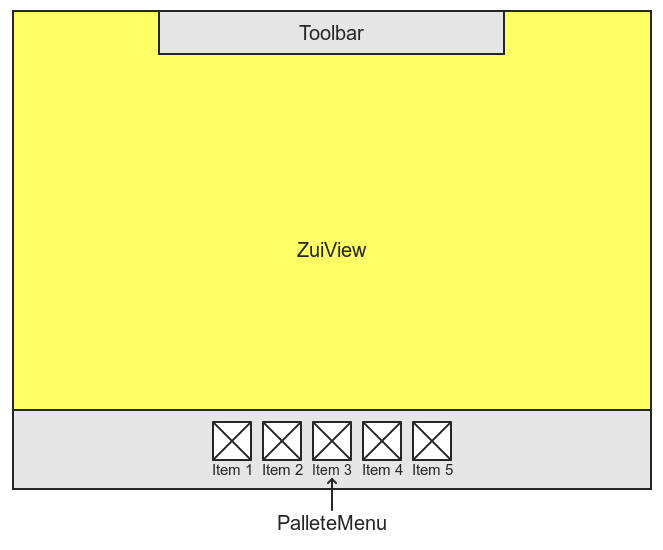
\includegraphics[width=0.75\textwidth]{editacia}} \\
 \subfloat[Prezentácia]{\label{fig:prezentacia}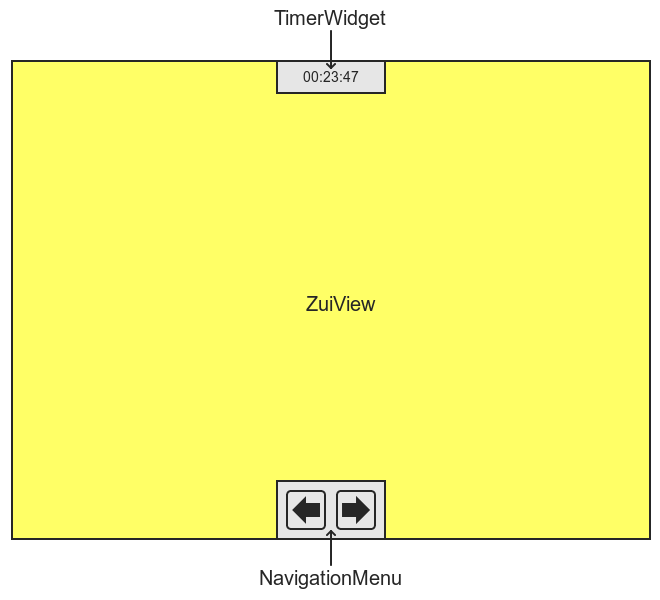
\includegraphics[width=0.75\textwidth]{prezentacia}}
 \caption{Používateľské rozhranie}
 \label{fig:ui}
\end{figure}

\chapter{Implementácia} \label{ch:implementacia}

\section{Qt}

Aplikáciu popísanú v kapitole \nameref{ch:navrh} sme sa rozhodli implementovať s využitím frameworku QtQuick. Tento framework nám ponúka vysokoúrovňové prostriedky, ktoré nám uľahčia celú implementáciu. V nasledujúcej časti popíšeme najdôležitejšie technológie, ktoré sme z tohto frameworku použili.

\subsection{Graphics View framework}

Framework \textit{Graphics View} ponúka prostriedky na vizualizáciu dát pomocou prístupu \textit{model-view}. Základnými triedami pre manipuláciu s týmto frameworkom sú \texttt{QGraphics\-Scene} a \texttt{QGraphicsView}.

Framework ponúka mnoho základných prvkov, ktoré sa dajú do scény vložiť a následne vykresliť cez \uv{pohľad} (\texttt{QGraphicsView}). Každý prvok v scéne má vlastný súradnicový systém, do ktorého vieme vložiť ďalšie prvky. Potomkovia nejakého prvku dedia transformačnú maticu aplikovanú na rodičov a pridávajú svoju vlastnú, čím sa dá dosiahnuť vysokej flexibility.

Vykresľovanie môže byť prevedené viacerými spôsobmi. Najpoužívanejšími sú rastrové vykresľovanie, ktoré je veľmi presné, ale je ale náročné na procesorový výkon počítaču a teda nie vhodné pre animácie. Druhým spôsobom je vykresľovanie cez OpenGL, ktoré je síce rýchle (ak neberieme v úvahu celú abstrakciu architektúry frameworku), no nemusí byť podporované na každej platforme.

\subsection{Qt Meta-object Language}

\textit{Qt Meta-object Language}, skrátene QML, je deklaratívny programovací jazyk inšpirovaný JavaScriptom, špeciálne navrhnutý na jednoduchý popis dynamických používateľských rozhraní. Každý QML dokument popisuje stromovú štruktúru elementov, ktoré obsahujú identifikátor, definície vlastností, funkcií, atď.

QML intenzívne využíva systém meta-objektov knižnice Qt. Tento mechanizmus zabezpečuje dôležitú vlastnosť jazyka, ktorým je tzv. \uv{property binding}, teda viazanie vlastností objektov. Ak je vlastnosť \texttt{foo} objektu \texttt{A} naviazaná na vlastnosť \texttt{bar} objektu \texttt{B}, tak pri zmene hodnoty \texttt{B.bar} sa automaticky zmení aj hodnota \texttt{A.foo}. Tento systém sa na prvý pohľad podobá použitiu smerníkov z iných jazykov, avšak hodnota vlastnosti objektu v jazyku QML môže byť akýkoľvek javascriptový výraz. Tento výraz sa automaticky vyhodnotí vždy keď dôjde k zmene zdrojovej hodnoty vlastnosti. Výpis \ref{lst:property_binding} znázorňuje jednoduché použitie tejto vlastnosti -- objekt \texttt{item2} si bude udržiavať dvojnásobnú veľkosť objektu \texttt{item1}.

\lstinputlisting[label=lst:property_binding, caption=Viazanie vlastností]{kod/property_binding.qml}

Okrem viazania vlastností, QML ponúka ďalšiu zaujímavú konštrukciu, ktorá umožňuje definovať stavy objektov a prechody medzi nimi. Stav objektu je množina hodnôt jeho vlastností a prechod určuje akým spôsobom sa mení samotná hodnota vlastnosti. Vo výpise \ref{lst:states_transitions} je možné vidieť definíciu objektu, ktorý má 2 stavy -- \textit{active} a \textit{inactive}. V aktívnom stave sa má zobrazovať ako úplne priehľadný a v normálnej veľkosti, pričom v neaktívnom stave, ktorý je prednastavený, ako polo-priehľadný a len s troj-štvrtinovou veľkosťou. Ak teda zmeníme stav objektu na jeden z definovaných, obe tieto vlastnosti zmenia svoju hodnotu na takú aká je priradená v žiadanom stave.

Nevýhodou tohto prístupu je okamžitá zmena hodnôt vlastností, čo nemusí byť vždy žiadané. Ak potrebujeme plynulú zmenu medzi definovanými hodnotami vlastnosti, môžeme využiť prechody medzi stavmi. V našom prípade vo výpise \ref{lst:states_transitions} je definovaný jeden prechod, ktorý sa sa automaticky použije na prechod z aktívneho na neaktívny stav a tiež opačne. Prechod obsahuje \uv{číselnú animáciu}, ktorá zaisťuje plynulú zmenu medzi číselnými hodnotami vďaka interpolácií medzi hodnotami vlastností z oboch stavov.

\lstinputlisting[label=lst:states_transitions, caption=Stavy a prechody]{kod/states_transitions.qml}

Definovanie animácií, nech už sú akokoľvek zložité, je v jazyku QML vskutku jednoduché. Vďaka deklaratívnemu prístupu jazyka môžeme vytvárať hierarchiu sekvenčných a paralelných skupín animácií.

\subsection{QtQuick}

\textit{QtQuick} označuje technológiu, ktorá umožňuje vytvárať vysoko dynamické používateľské rozhrania deklaratívnou cestou. Základným kameňom celého frameworku je jazyk QML, spolu s grafickými, ale aj negrafickými elementami, ktoré vieme vytvárať pomocou tohto jazyka.

\subsubsection{Elementy}

Medzi základné grafické prvky patria napr. \texttt{Rectangle}, \texttt{Image}, \texttt{BorderImage}, \texttt{Animated\-Image}, \texttt{Gradient} alebo aj \texttt{Text}. Interakcia s používateľom je riešená veľmi netradične, pomocou nevizuálnych elementov ako \texttt{MouseArea} (stará sa o pohyb a tlačidlá myši), \texttt{Keys} (riadi vstup z klávesnice), \texttt{PinchArea} (využíva viacdotykové vstupné zariadenia) a ďalších. Existuje mnoho ďalších elementov, ktoré ponúka tento framework, že ich popis by bol sa samostatnú prácu.

\subsubsection{Verzie}

Prvá verzia toto frameworku, teda \textit{QtQuick 1.0}, je implementovaná pomocou tried z frameworku \textit{Graphics View}, ktorý sme popísali v tejto časti. Táto skutočnosť nám dovoľuje jednoducho rozširovať funkcionalitu o nami definované deklaratívne objekty, ktoré môžeme používať priamo z QML. Hoci je táto implementácia aktívne podporovaná a chystá sa revízia 1.1, je známe, že v piatej verzií frameworku Qt bude nahradená verziou 2.0.

Framework \textit{QtQuick 2.0} má s predchádzajúcou verziou len málo spoločné. Hoci sa API (\textit{Application Programming Interface}, v preklade \uv{rozhranie pre programovanie aplikácií}) nezmení (stačí v aplikácií importovať novú verziu), implementácia je úplne odlišná. Tá používa namiesto abstrakcie v podobe \textit{Graphics View}, priame vykresľovanie pomocou OpenGL volaní. Hlavným dôvodom pre túto zmenu bola snaha dosiahnuť čo najlepší výkon, ktorý je žiadaný najmä na mobilných zariadeniach.

\section{Popis implementácie}

Vďaka kvalitnému návrhu práce, sme mali s implementáciou veľmi málo problémov. V~tejto časti stručne popíšeme rozdiely oproti návrhu, ktoré nám spôsobili problémy.

\subsection{Animácia prechodu}

Aj napriek tomu, že sme predpokladali, že s najzložitejšou časťou aplikácie-- animáciou prechodu, nastanú problémy, nič také sa neudialo. Problémy nenastali vďaka deklaratívnemu prístupu frameworku \textit{QtQuick}, s ktorým je implementácia podobných typov algoritmov priamočiara. Jediným problémom, ktorý počas programovania tejto časti nastal, bolo nekorektné správanie animácie pri vyžiadaní animácie na ďalší objekt, ak už animácia bežala. Tento problém sme vyriešili miernou zmenou algoritmu, ktorý pri novej animácií berie v úvahu aktuálnu pozíciu kamery a pokračuje z tohto aktuálneho bodu.

\subsection{Export plátna}

Pravdepodobne najväčšou prekážkou bol jeden z cieľov práce, a to export celého plátna do vybraného formátu. Ako je napísané v úvode tejto kapitoly, rozhodli sme sa túto aplikáciu implementovať vo frameworku \textit{QtQuick} v jazyku QML. Obe tieto technológie sú ešte nevyzreté a vývoj stále prebieha, čo má za následok isté obmedzenia. Príkladom takéhoto obmedzenia je nemožnosť pristupovať k nízkoúrovňovej reprezentácií samotných objektov -- pixelom. Riešením tohto problému bolo vytvorenie C++ zásuvného modulu do \textit{QtQuick}, ktorý poskytoval QML rozhranie pre požadovanú funkcionalitu. Aj napriek tomu, že toto riešenie funguje, tento modul nie je kompatibilný s \textit{QtQuick} 2.0, čo znemožňuje využiť v budúcnosti lepšie vykresľovanie, ktoré táto verzia prinesie.

\subsection{Používateľské rozhranie}

Vďaka \textit{QtQuick} sme vytvorili používateľské rozhranie bez najmenších problémov. Hoci sa jedná o veľmi jednoduché rozhranie, v ktorom je dostupných pomerne málo funkcií, svojmu účelu slúži dobre. Demonštráciu rozhrania v prezentačnom móde je možné vidieť na obrázku \ref{fig:mfp}. Ako sme uviedli v návrhu práce, panely s akciami sú normálne skryté. Až po ich aktivácií sa animáciou vysunú a po použití sa naspäť plynulo zasunú.

Nepríjemnou vlastnosťou programu je nutnosť použiť softvérové vykresľovanie na dosiahnutie prijateľného grafického výstupu.

\begin{figure}
 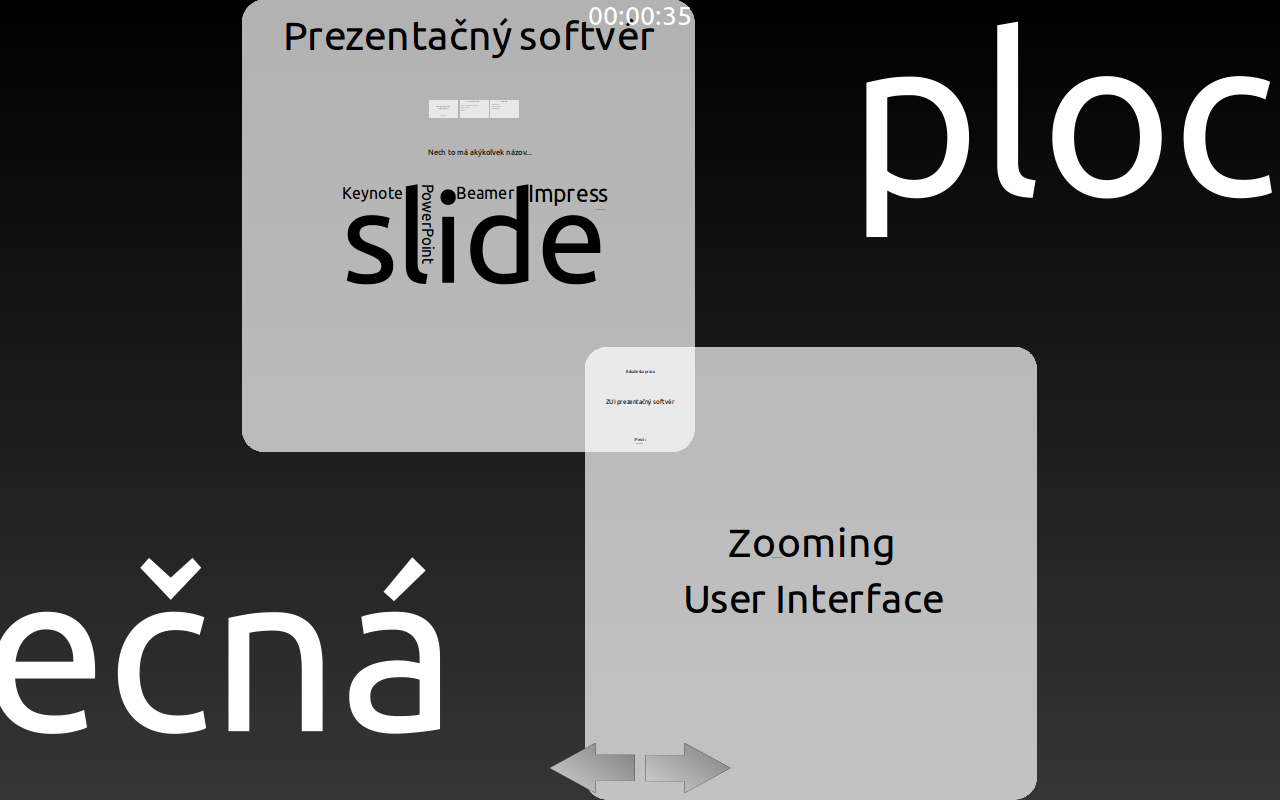
\includegraphics[width=\linewidth]{mfp}
 \caption{Ukážka bežiacej prezentácie\label{fig:mfp}} 
\end{figure}

\chapter{Zhodnotenie} \label{ch:zhodnotenie}

Táto práca nám poskytla mnoho teoretických, ale najmä praktických poznatkov, ktoré sme pri jej tvorení osvojili. Umožnila nám preskúmať netradičný, no o to zaujímavejší typ používateľského rozhrania -- \textit{Zooming User Interface}. Implementovali sme sofistikovanú animáciu, určenú na príjemné sledovanie a navigáciu v takýchto rozhraniach. A do tretice sme objavili výhody, avšak aj slabiny frameworku \textit{QtQuick}.

Výsledkom tejto bakalárskej práce je jednoduchý nástroj na vytváranie a prehrávanie prezentácií na báze \textit{Zooming User Interface}. Ciele, ktoré sme mali stanovené, sa nám podarilo zväčša naplniť. Aplikáciu sme dokonca otestovali aj v reálnych podmienkach -- pri ozajstnej prezentácií. Tento test potvrdil, že aj napriek svojej jednoduchosti, je výsledná aplikácia použiteľná.

Aj napriek tomu, že aplikácia prešla testom použiteľnosti, neznamená to, že je hotová. Existuje ešte veľký priestor na vylepšenie. V budúcnosti bude možné vďaka novej verzií \textit{QtQuick}, použiť viacvláknové vykresľovanie cez OpenGL, ktoré ponúkne lepší výkon a kvalitnejší výstup. Rozhranie pre tvorbu prezentácií by mohlo byť omnoho intuitívnejšie a obsahovať viac funkcií. Zaujímavou možnosťou by bolo preskúmať použitie ZUI pre iné typy aplikácií, či dokonca ako hlavné používateľské rozhranie operačného systému, na stolových počítačoch alebo mobilných zariadeniach.